\documentclass[12pt, a4paper]{report}

\usepackage{geometry}
\geometry{a4paper, left=30mm, right=20mm, top=30mm, bottom=30mm}

\usepackage{t1enc}
\usepackage[utf8]{inputenc}
\usepackage[magyar]{babel}
\usepackage{amsmath}
\usepackage{amsfonts}
\usepackage{algorithm}
\usepackage{algpseudocode}
\usepackage{amsthm}
\usepackage{listings}
\usepackage{color}
\usepackage{xcolor}
\usepackage{colortbl}
\usepackage{caption}
\usepackage{subcaption}
\usepackage{ellipsis}
\usepackage{multirow}
\usepackage{tocloft}

\usepackage[autostyle]{csquotes}
\selectlanguage{magyar}
\DeclareQuoteAlias{dutch}{magyar}

\usepackage{apacite}
\bibliographystyle{apacite}

\usepackage{url}
\usepackage{textcomp}

\usepackage{tikz}
\usetikzlibrary{shapes}
\usetikzlibrary{positioning}

\usepackage[decimalsymbol=comma]{siunitx}

\usepackage[linewidth=0.33pt, rightline=false, leftline=false, framemethod=tikz]{mdframed}

\usepackage{graphicx}
\graphicspath{ {./images/} }

% Különleges karakterek használatának lehetősége kódrészletben
\lstset{literate=
 {á}{{\'a}}1 {é}{{\'e}}1 {í}{{\'i}}1 {ó}{{\'o}}1 {ú}{{\'u}}1
 {Á}{{\'A}}1 {É}{{\'E}}1 {Í}{{\'I}}1 {Ó}{{\'O}}1 {Ú}{{\'U}}1
 {ö}{{\"o}}1 {ü}{{\"u}}1 {Ö}{{\"O}}1 {Ü}{{\"U}}1
 {ű}{{\H{u}}}1 {Ű}{{\H{U}}}1 {ő}{{\H{o}}}1 {Ő}{{\H{O}}}1
}

% A kódrészletek beállításai
\definecolor{codegray}{rgb}{0.5,0.5,0.5}
\lstset{xleftmargin=15pt,
        basicstyle=\scriptsize,
        numbers=left,
        numbersep=5pt,
        numberstyle=\tiny\color{codegray},
        escapechar=@,
        aboveskip=2em,
        belowskip=2em,
        belowcaptionskip=2em}

% JS nyelv
\lstdefinelanguage{JavaScript}{
  keywords={typeof, new, true, false, catch, function, return, null, catch, switch, var, if, while, do, else, case, break, yield, let, const, await, async},
  keywordstyle=\bfseries,
  ndkeywords={class, export, boolean, throw, implements, import, this},
  ndkeywordstyle=\bfseries,
  identifierstyle=\color{black},
  sensitive=false,
  comment=[l]{//},
  morecomment=[s]{/*}{*/},
  commentstyle=\ttfamily,
  stringstyle=\ttfamily,
  morestring=[b]',
  morestring=[b]",
  morestring=[b]`
}

\lstdefinelanguage{WebIDL}{
  keywords={interface, enum, class, dictionary, typedef},
  keywordstyle=\bfseries,
  ndkeywordstyle=\bfseries,
  identifierstyle=\color{black},
  sensitive=false,
  comment=[l]{//},
  morecomment=[s]{/*}{*/},
  commentstyle=\ttfamily,
  stringstyle=\ttfamily,
  morestring=[b]',
  morestring=[b]"
}

% Fix listings
\renewcommand{\lstlistingname}{Kódrészlet}

% Fix APA
\renewcommand\BOthers{és mtsai\hbox{}}
\renewcommand\BOthersPeriod{és mtsai.\hbox{}}
\renewcommand\BRetrievedFrom{Letöltve:\ }
\renewcommand\BRetrieved[1]{Letöltve, {#1}:\ }
\renewcommand\BIn{}
\renewcommand\BED{Szerk. \hbox{}}
\renewcommand\BEDS{Szerk. \hbox{}}
\renewcommand\BMTh{Diplomamunka}
\renewcommand{\BCBT}{}
\renewcommand{\BCBL}{}

\renewcommand{\ellipsisgap}{0.1em}

% 1,5-es sorköz
\linespread{1.25}

\providecommand{\useColors}{1}

\newtheorem*{definition*}{Definíció}

\providecommand*{\printsecond}[2]{#2}

\renewcommand\cftchapafterpnum{\vskip2pt}

\newcommand{\dotref}[1] {\ref{#1}.}

\newenvironment{outdentlist}
  {\begin{list}{}{\setlength\itemindent{-\leftmargin}}}
  {\end{list}}


\theoremstyle{definition}
\newtheorem{definition}{Definíció}

\begin{document}
    \if\printName1
        \begin{titlepage}

\center
\vspace*{7.5cm}
{\huge \bfseries TDK dolgozat}\\[0.5cm]

{\LARGE Szerzők: Bagossy Attila, Vécsi Ádám}

\vfill

\end{titlepage}

    \fi
    % University Assignment Title Page 
% LaTeX Template
% Version 1.0 (27/12/12)
%
% This template has been downloaded from:
% http://www.LaTeXTemplates.com
%
% Original author:
% WikiBooks (http://en.wikibooks.org/wiki/LaTeX/Title_Creation)
%
% License:
% CC BY-NC-SA 3.0 (http://creativecommons.org/licenses/by-nc-sa/3.0/)

\begin{titlepage}

\center

\textsc{\LARGE Debreceni Egyetem}\\[1.5cm]
\textsc{\Large Informatikai Kar}
\\[0.5cm]

\textsc{\large Számítógéptudományi Tanszék}
\\[2.5cm]

{\huge \bfseries CryptID – Platformfüggetlen Identity-based Encryption megoldás \par}

\if\printName1
  \vspace*{6.5cm}

  \begin{minipage}{.4\linewidth}
    \begin{flushleft}
      \large \textit{Témavezető:} \\
      Dr. Pethő Attila  \\
      egyetemi tanár
    \end{flushleft}
  \end{minipage}
  \hfill
  \begin{minipage}{.52\linewidth} 
    \begin{flushright}
      \large \textit{Szerzők:}\\
      Bagossy Attila, \textit{PTI MSc, 2. évfolyam} \\
      Vécsi Ádám, \textit{PTI MSc, 2. évfolyam}
    \end{flushright}
  \end{minipage}
  \\[2.5cm]
\else
  \vspace*{10.5cm}
\fi

{\large Lezárva: 2019. 01. 05.}\\ 

\vfill

\end{titlepage}

    \setlength{\cftbeforechapskip}{.2ex}
    \setlength{\cftbeforesecskip}{-.5ex}
    \tableofcontents

    \chapter*{Köszönetnyilvánítás}
\addcontentsline{toc}{chapter}{Köszönetnyilvánítás}

\if\printName1

Szeretnénk megköszönni a dolgozat elkészítésében nyújtott segítséget a témavezetőnknek, Dr. Pethő Attilának. Az elmúlt hónapokban megannyi személyes egyeztetés és levélváltás során látott el minket nélkülözhetetlen szakmai tanácsokkal.

\hfill\break
\hfill\break

\fi

A kutatást a „Integrált kutatói utánpótlás-képzési program az informatika és számítástudomány diszciplináris területein” (EFOP-3.6.3-VEKOP-16-2017-00002) című projekt támogatta. 
A projekt a Magyar Kormány és az Európai Szociális Alap társfinanszírozásában valósult meg.

\begin{figure}[b]
    \hbox{\hspace{26em} 
\includegraphics[scale=0.1]{efop-logo.jpg}}
\end{figure}


    \chapter{Bevezetés}

A dolgozatunkban az általunk fejlesztett CryptID Identity-based Encryption (IBE) könyvtárat mutatjuk be. Ez a Boneh-Franklin IBE egy újszerű implementációja, mely reményeink szerint nemcsak egy újabb megvalósítás, hanem valóban olyan jellemzőkkel bír, melyek a már rendelkezésre álló megoldások versenytársává avathatják. Ehhez természetesen olyan sajátosságok szükségesek, melyek megkülönböztetik a többi könyvtártól, mi több, bizonyos összevetésben azok elé helyezik. Úgy gondoljuk, hogy a platformfüggetlen működés, a strukturált publikus kulcs és a fejlesztő-orientált interfész ilyenek lehetnek.

\section{Identity-based Encryption}

A nyilvános kulcsú kriptográfia egy fiatal ága az IBE, melynek ötletét Adi Shamir fogalmazta meg 1984-ben. Egy olyan sémát írt le, melyben nincsen szükség sem a nyilvános, sem a titkos kulcsok előzetes cseréjére vagy nyilvántartására: a nyilvános kulcsok egyértelmű, mindenki által ismert azonosítók (például egy telefonszám), míg a titkos kulcsokat egy megbízható harmadik fél, a Private Key Generator (PKG) hozza létre. Ekképpen az IBE nem igényel a Public Key Infrastructure-höz (PKI) hasonló rendszert a kulcsok kezeléséhez, hiszen az adatok titkosításához szükséges kulcsokat a rendszer minden résztvevője ismeri, a visszafejtéshez pedig egyetlen féllel, a PKG-vel kell kapcsolatba lépni. Habár utóbbi aggályos lehet, hiszen a felhasználóknak nincsen befolyása a titkos kulcs előállítására, azonban ezt a feladatot a PKI esetén is egy külső fél, a \textit{registration authority} (RA) végzi \cite{Buchmann::IntroductionToPublicKeyInfrastructures}. 

Az IBE gyakorlatban is használható első leírását Boneh és Franklin adta 2001-ben. Ez a rendszer azonban csak az első volt a sorban: napjainkig számos különböző IBE-rendszer született meg, melyek rendre eltérő jellemzőkkel rendelkeznek. Az elméleti előrelépéseket követte a gyakorlat is, hiszen a fejlesztők mára több implementáció közül is választhatnak.

\section{Motiváció}

Az internetre csatlakozó mobil eszközök robbanásszerű elterjedése igényt ébresztett hatékony és hordozható kriptográfiai rutinok iránt. Ugyanakkor a jelenlegi megvalósítások egyáltalán nem, vagy csak kevésbé veszik figyelembe ezt az igényt. Emiatt a CryptID kifejezetten a platformfüggetlenséget szem előtt tartva készült, legyen szó asztali, mobil vagy IoT eszközökről.

A publikus kulcsban elhelyezhető metaadatok ötlete már Boneh és Franklin cikkében is megjelenik \citeyear{Boneh::IdentityBasedEncryptionFromTheWeilPairing}. Az elképzelés lényege, hogy az azonosítón felül további adatokat, például egy dátumot is elhelyezünk a publikus kulcsban. Az elképzelést annyira előremutatónak találtuk, hogy a CryptID ehhez teljes mértékű támogatást biztosít – a publikus kulcsok ugyanis JSON objektumokként reprezentálhatók.

Mi motiválta viszont a fejlesztő-orientált interfész létrehozását? Az ismert könyvtárakat áttekintve azt vettük észre, hogy bár nagyszerű kriptográfiai képességekkel rendelkeznek, azonban helyes működtetésükhöz számottevő matematikai és kriptográfiai háttér szükséges. Annak érdekében, hogy az IBE-t több fejlesztő tudja helyesen integrálni, a \mbox{Google} Tinkkel\footnote{\url{https://github.com/google/tink}} azonos mottót választva egy olyan könyvtár elkészítését tűztük ki célul, melyet könnyű jól használni és nehéz (vagy nehezebb) rosszul.

\section{A dolgozat felépítése}

A dolgozatunk első három fejezete bevezető jellegű: előbb az elliptikus görbe kriptográfián, valamint az IBE-n keresztül a matematikai alapokat tárgyaljuk, majd a WebAssembly formájában a technológiai hátteret ismertetjük. Ezt követi a dolgozat fő eredményét jelentő CryptID könyvtár rétegről rétegre történő részletes bemutatása, kiemelt figyelmet szentelve a teljesítmény elemzésének. Zárásként két alkalmazás szerepel, melyek a Crypt\-ID nagyobb léptékű programokba történő integrálását demonstrálják.

    \chapter{Elliptikus görbe kriptográfia}
\label{Chapter::ECC}

A fejezet célja, hogy bemutassa az Identity-based Encryption (IBE) megértéséhez szükséges matematikai hátteret. Ismerteti az elliptikus görbék matematikai elméletének felhasználását és szerepét a kriptográfiában. A fejezet elkészítéséhez Hankerson és munkatársai művét vettük alapul \citeyear{GuideToEllipticCurveCryptography}.

\section{Elliptikus görbék}

Az elliptikus görbékkel kapcsolatban rengeteg forrás létezik, hiszen már évszázadok óta tanulmányozzák matematikusok. Ahogyan azt Lang írta: \enquote{\textit{It is possible to write endlessly on Elliptic Curves (This is not a threat).}} \citeyear{Lang::EllipticCurve}. Ezzel szemben dolgozatunkban egy lényegre törő rövid áttekintést szeretnénk adni.
\\

Egy $\mathbb{F}$ test feletti elliptikus görbét azok a $P = (x, y) \in \mathbb{F}^2$ pontok alkotnak, amelyek kielégítik az alábbi egyenletet: $$y^2 + axy + by = x^3 + cx^2 + dx + e,$$ ahol $a, b, c, d, e, x, y \in \mathbb{F}$ és $a, b, c, d, e$ adottak. Az elliptikus görbék algebrai elméletéhez szükségünk van egy olyan képzetes, végtelen távoli $O$ pontra, amely rajta van minden függőleges egyenesen és az $x$-tengelyre vonatkozó tükörgépe önmaga, tehát $O = -O$.

A kriptográfiában kiemelt szereppel bírnak az úgynevezett Weierstrass elliptikus görbék \cite{Kobitz::ECC}, melyek egyenlete egyszerűbb az előbb látottnál: $$y^2 = x^3 + ax + b.$$ Egy ilyen görbéről látható példa a \dotref{Figure::ECC::EllipticCurve} ábrán. A dolgozat további részében is ilyen görbéket fogunk tekinteni.

\begin{figure}[H]
    \centering
    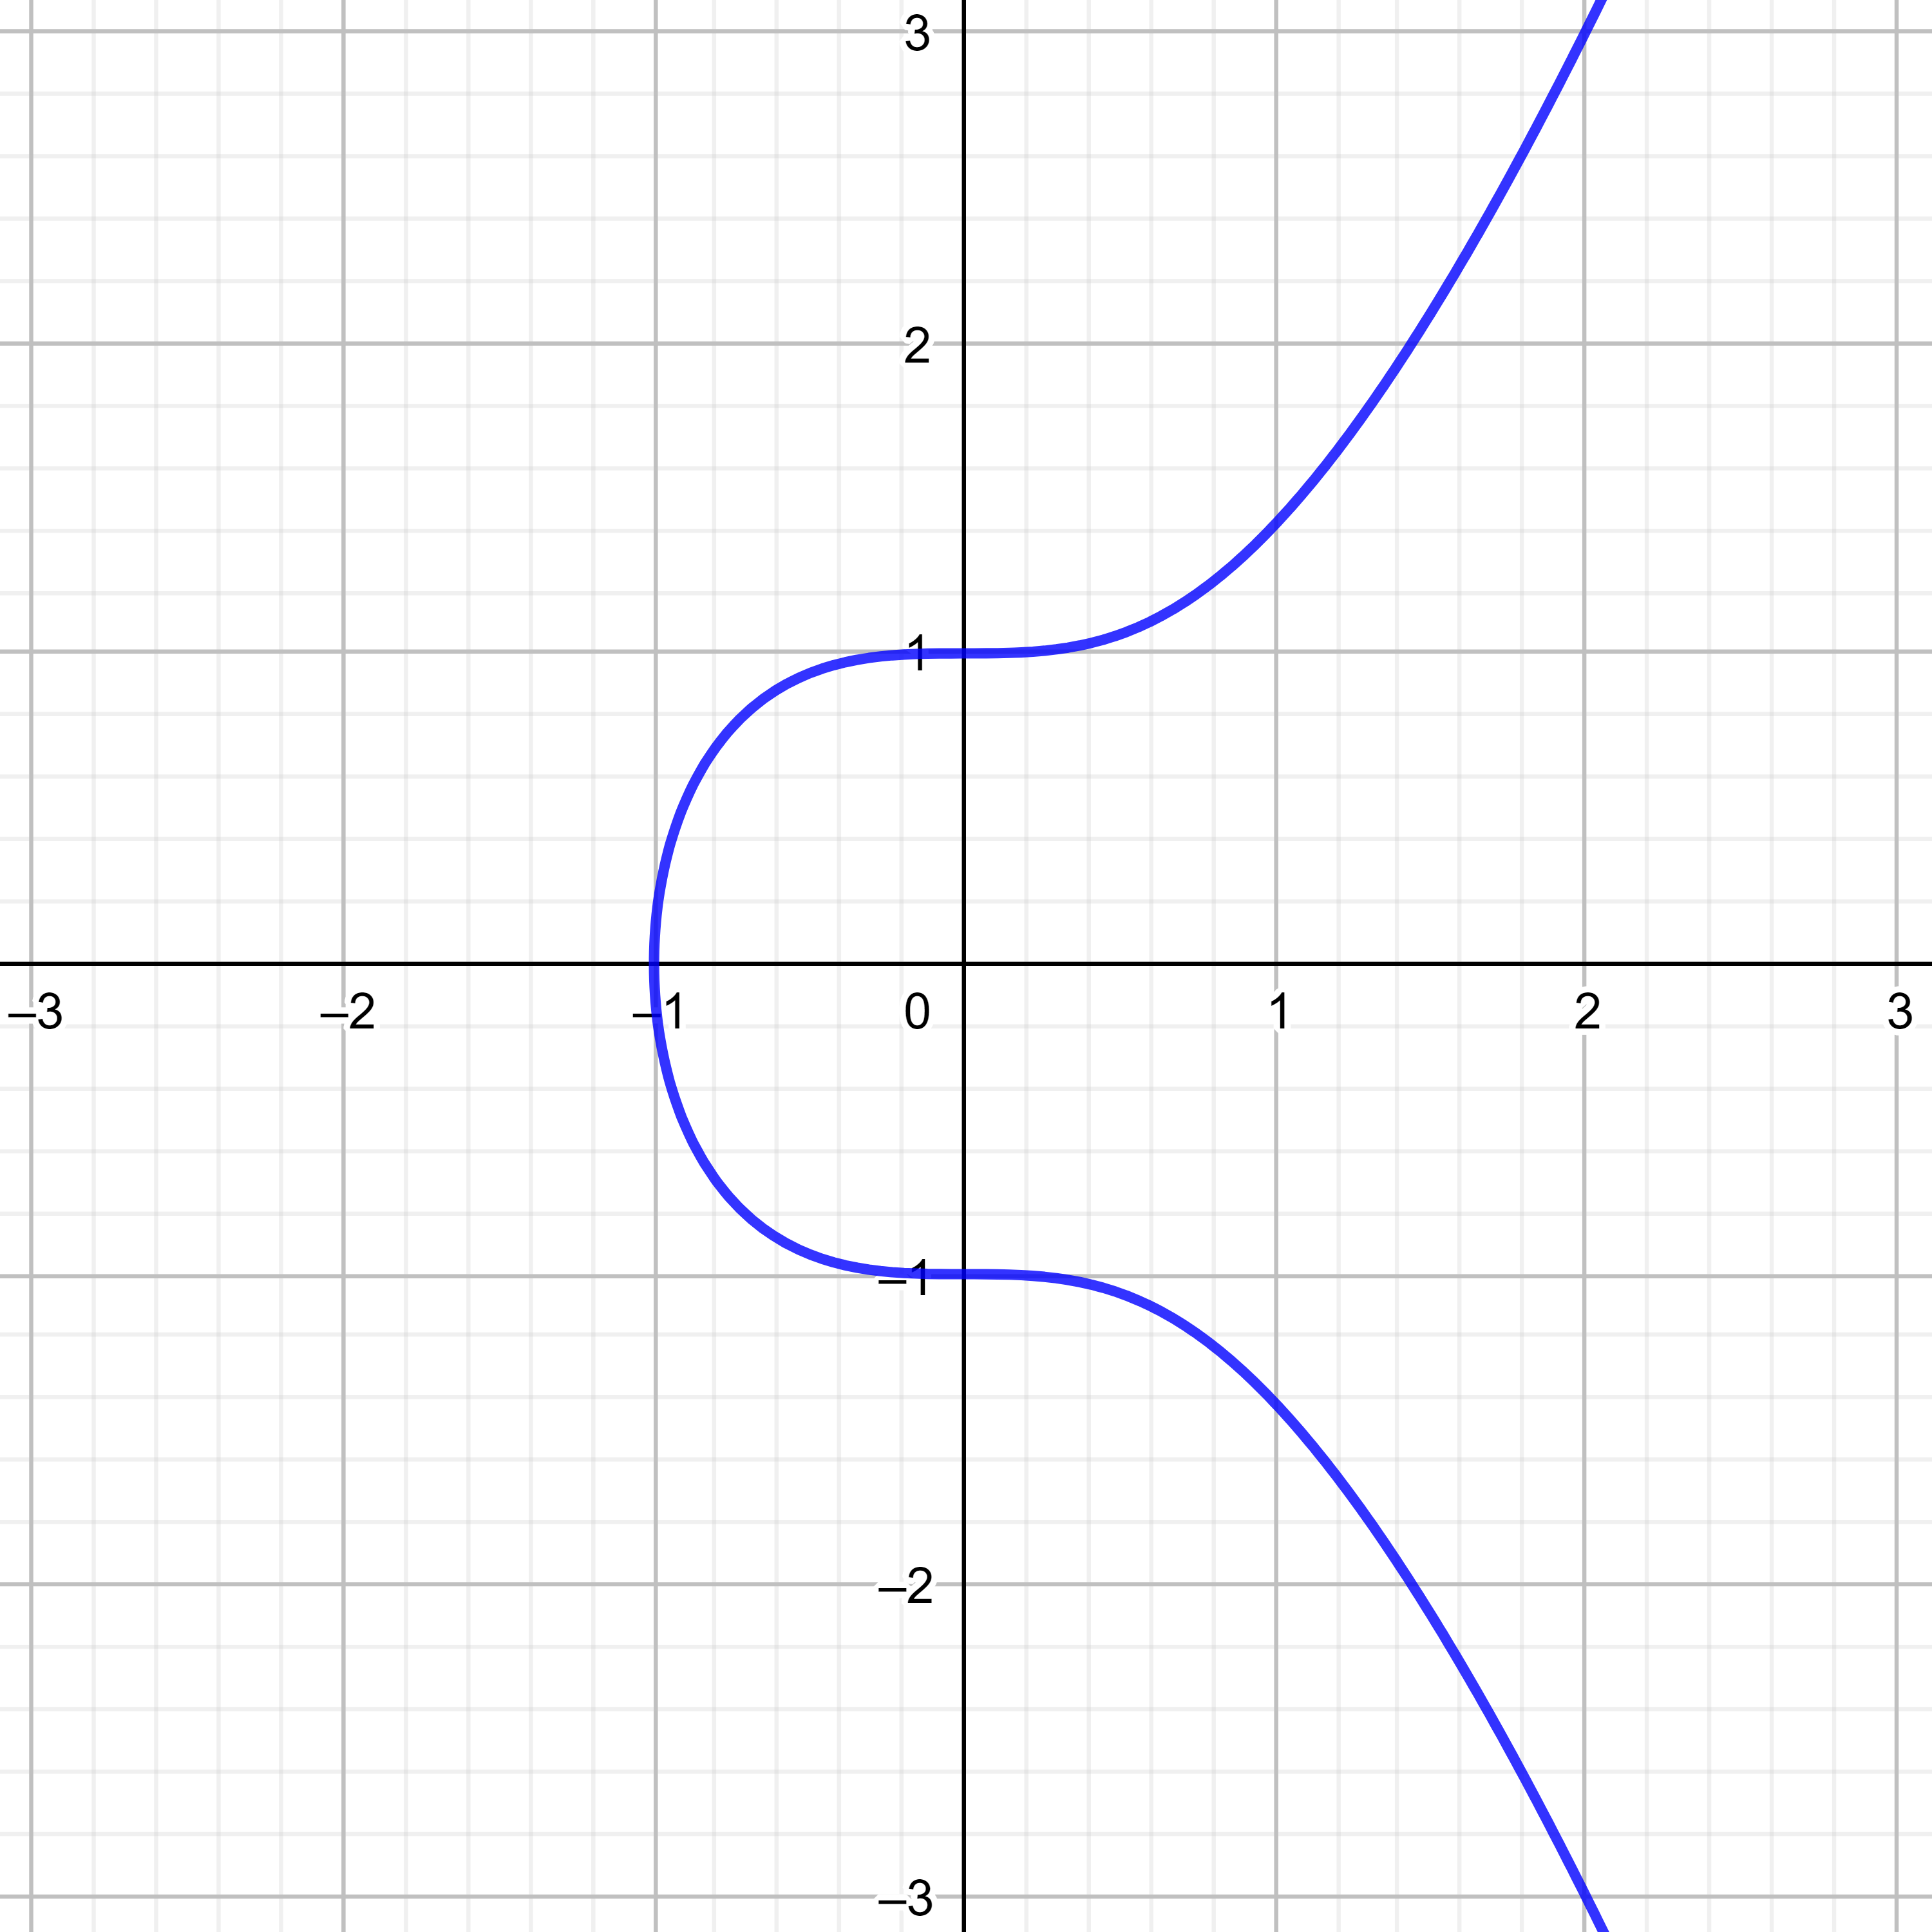
\includegraphics[width=0.4\textwidth]{02-elliptikus-gorbe-kriptografia/elliptikus-gorbe.png}
    \caption{Az $y^2 = x^3 + 1$ görbe a valós számok teste felett.}
    \label{Figure::ECC::EllipticCurve}
\end{figure}

\section{Műveletek elliptikus görbék pontjaival}

Az elliptikus görbék egy fontos tulajdonsága, hogy a görbe pontjai a megfelelően definiált összeadás művelettel Abel-csoportot alkotnak, amelyben az egységelem a korábban definiált $O$ végtelen távoli pont.

\subsection{Két pont összeadása}

Az összeadás szabályát geometriai úton a következőképp tekintjük. Legyen $E$ egy elliptikus görbe egy $K$ test felett, melynek jelölése $E(K)$. Legyen $P = (x_1, y_1)$ és $Q = (x_2, y_2)$ az $E$ elliptikus görbének két különböző pontja. Ekkor a $P$ és $Q$ pontok $R$ összegét a következő módon kapjuk.

Először húzzuk be a $P$-re és $Q$-ra illeszkedő egyenest. Ez az egyenes metszeni fogja az elliptikus görbét egy harmadik pontban. Ha ezt a harmadik pontot tükrözzük az $x$-tengelyre, akkor megkapjuk $R$-t. Adott pont önmagával vett összeadása (azaz duplázása) annyiban tér el az előzőtől, hogy egy olyan egyenest szükséges felrajzolni első lépésként, amely az elliptikus görbét az adott pontban érinti.

% Szándékosan van \ref és nem \dotref!
% A 2.2a és 2.2b után ugyanis nem kell pont.
Az előbbiekben leírt módszereket ábrázolják a \ref{Figure::ECC::EllipticCurveAddition1} és \ref{Figure::ECC::EllipticCurveAddition2} ábrák.

\begin{figure}[H]{}
    \centering
    \begin{subfigure}[t]{0.48\textwidth}
        \centering
        \captionsetup{width=.86\linewidth}
        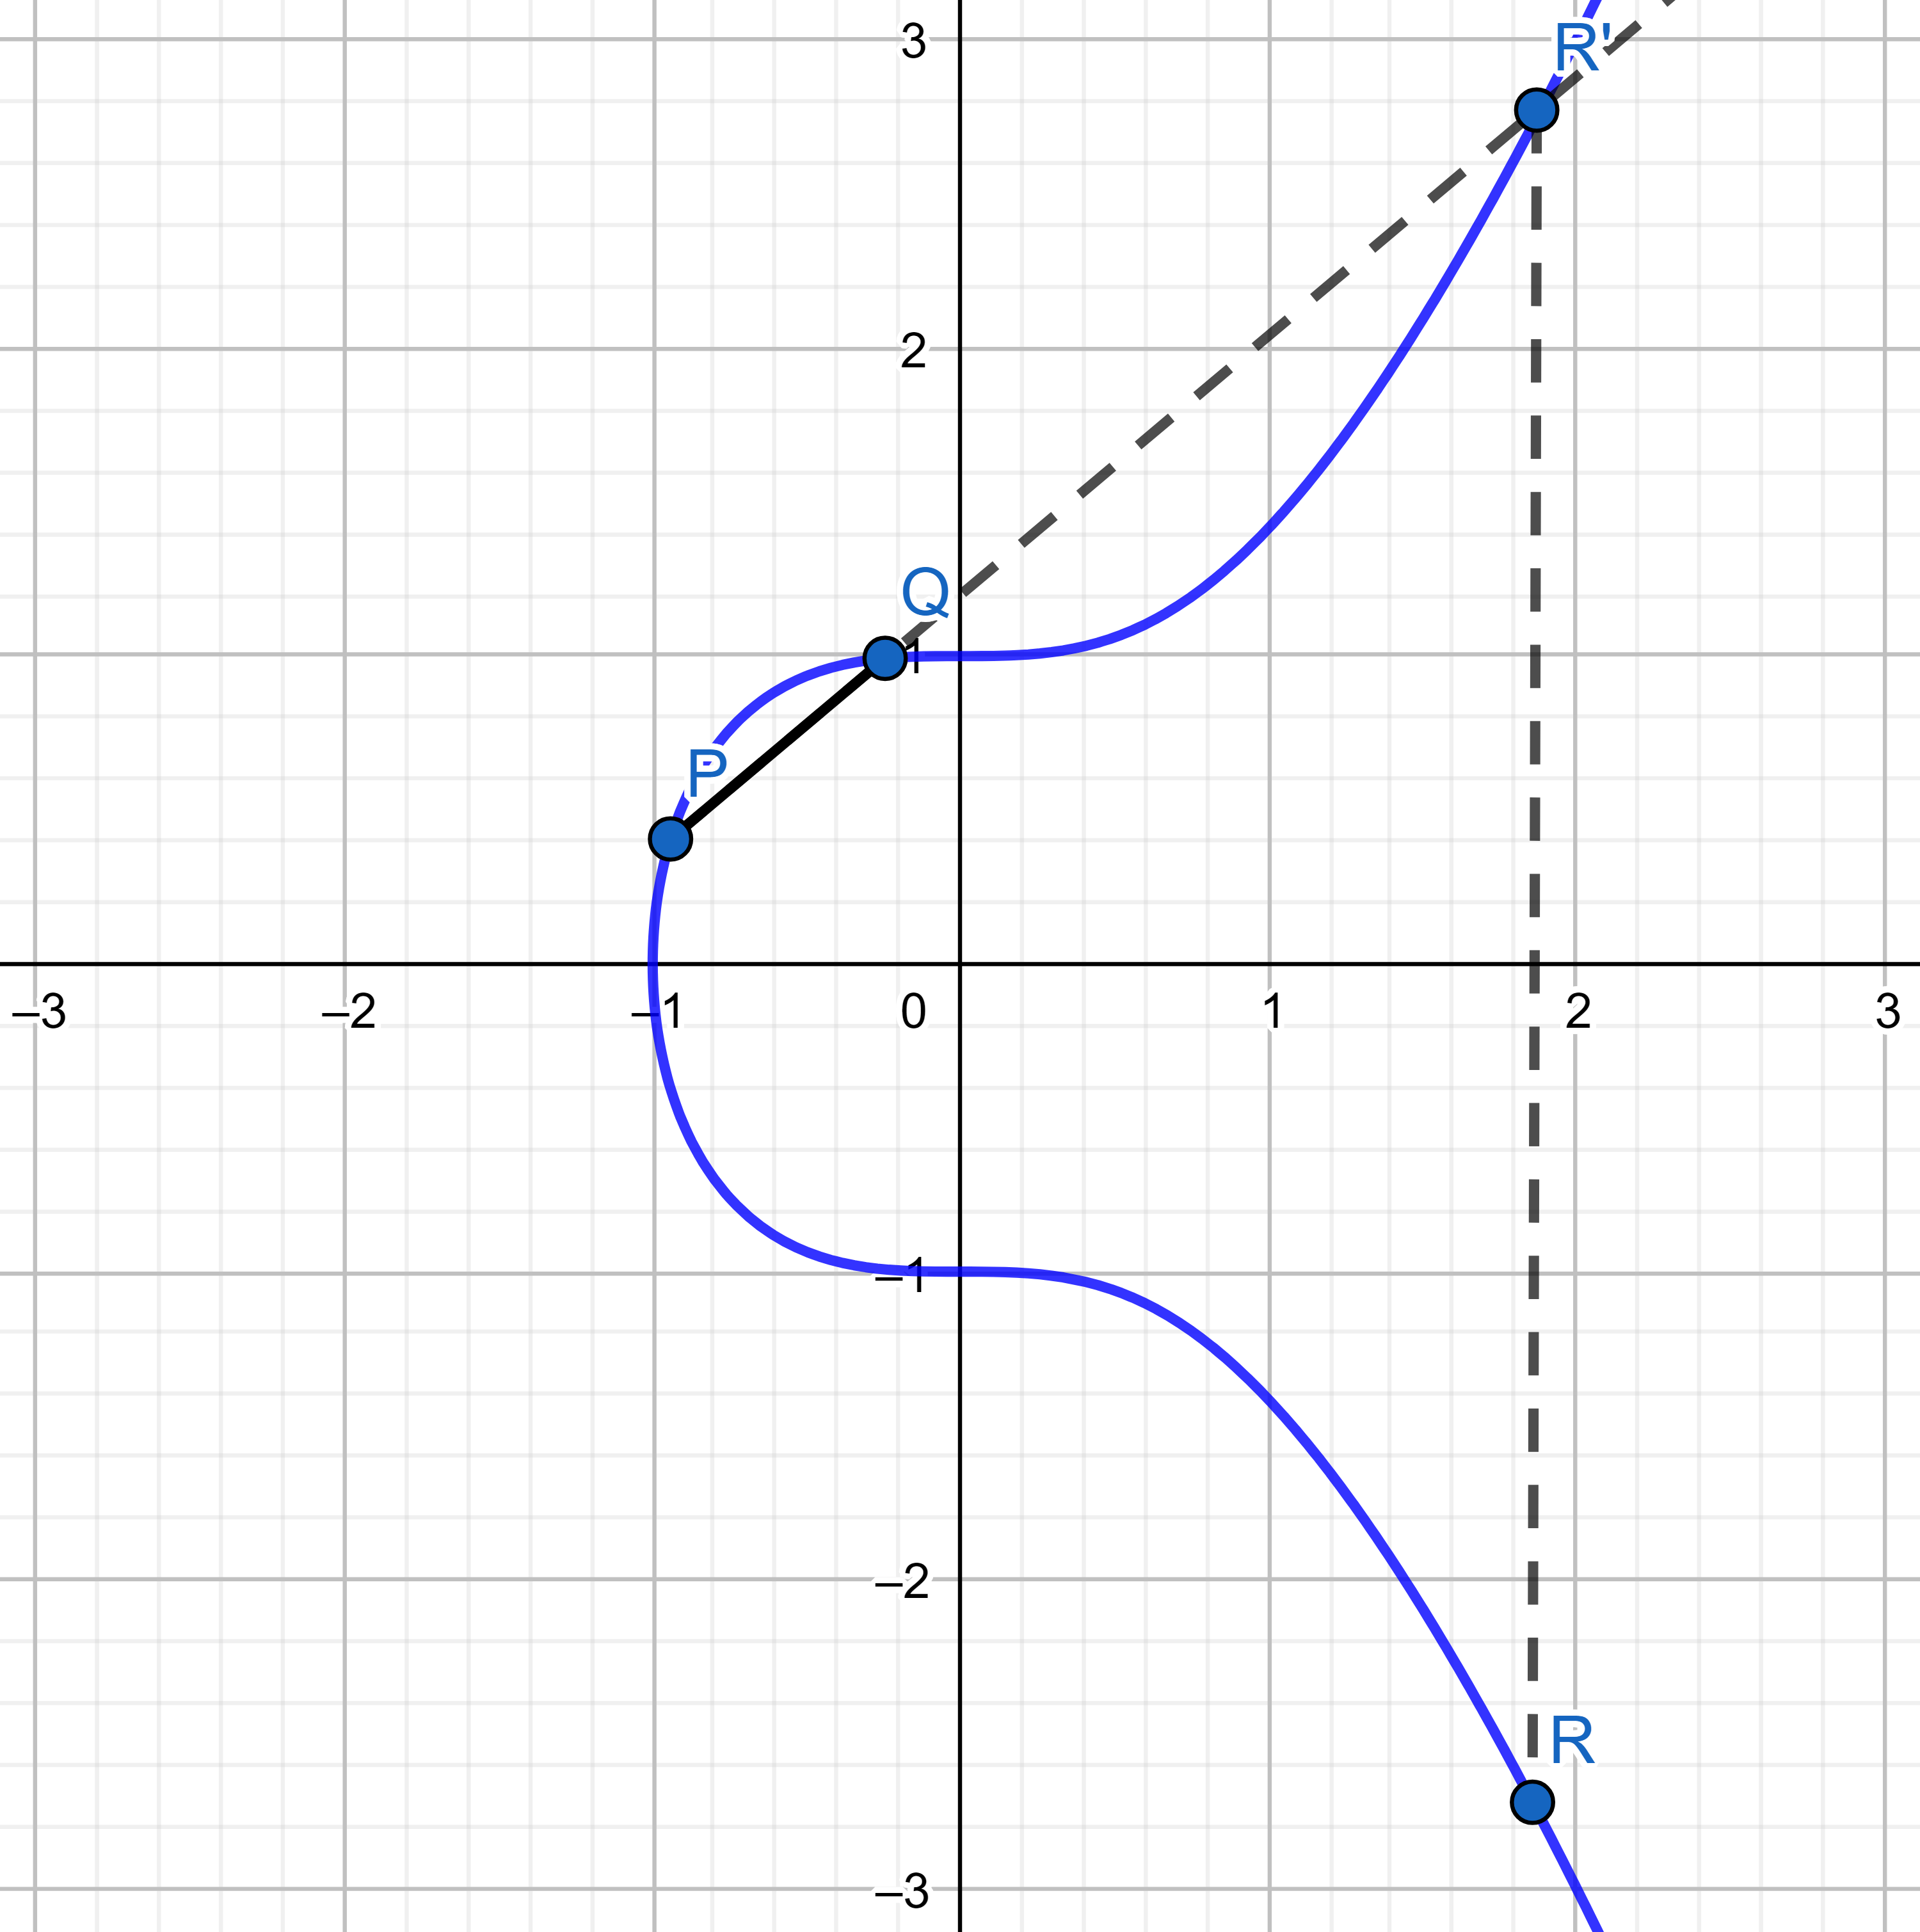
\includegraphics[width=.9\textwidth]{02-elliptikus-gorbe-kriptografia/elliptikus-gorbe-osszeadas1.png}
        \caption{Elliptikus görbe két különböző pontjának összeadása.}
        \label{Figure::ECC::EllipticCurveAddition1}
    \end{subfigure}
    \begin{subfigure}[t]{0.48\textwidth}
        \centering
        \captionsetup{width=.86\linewidth}
        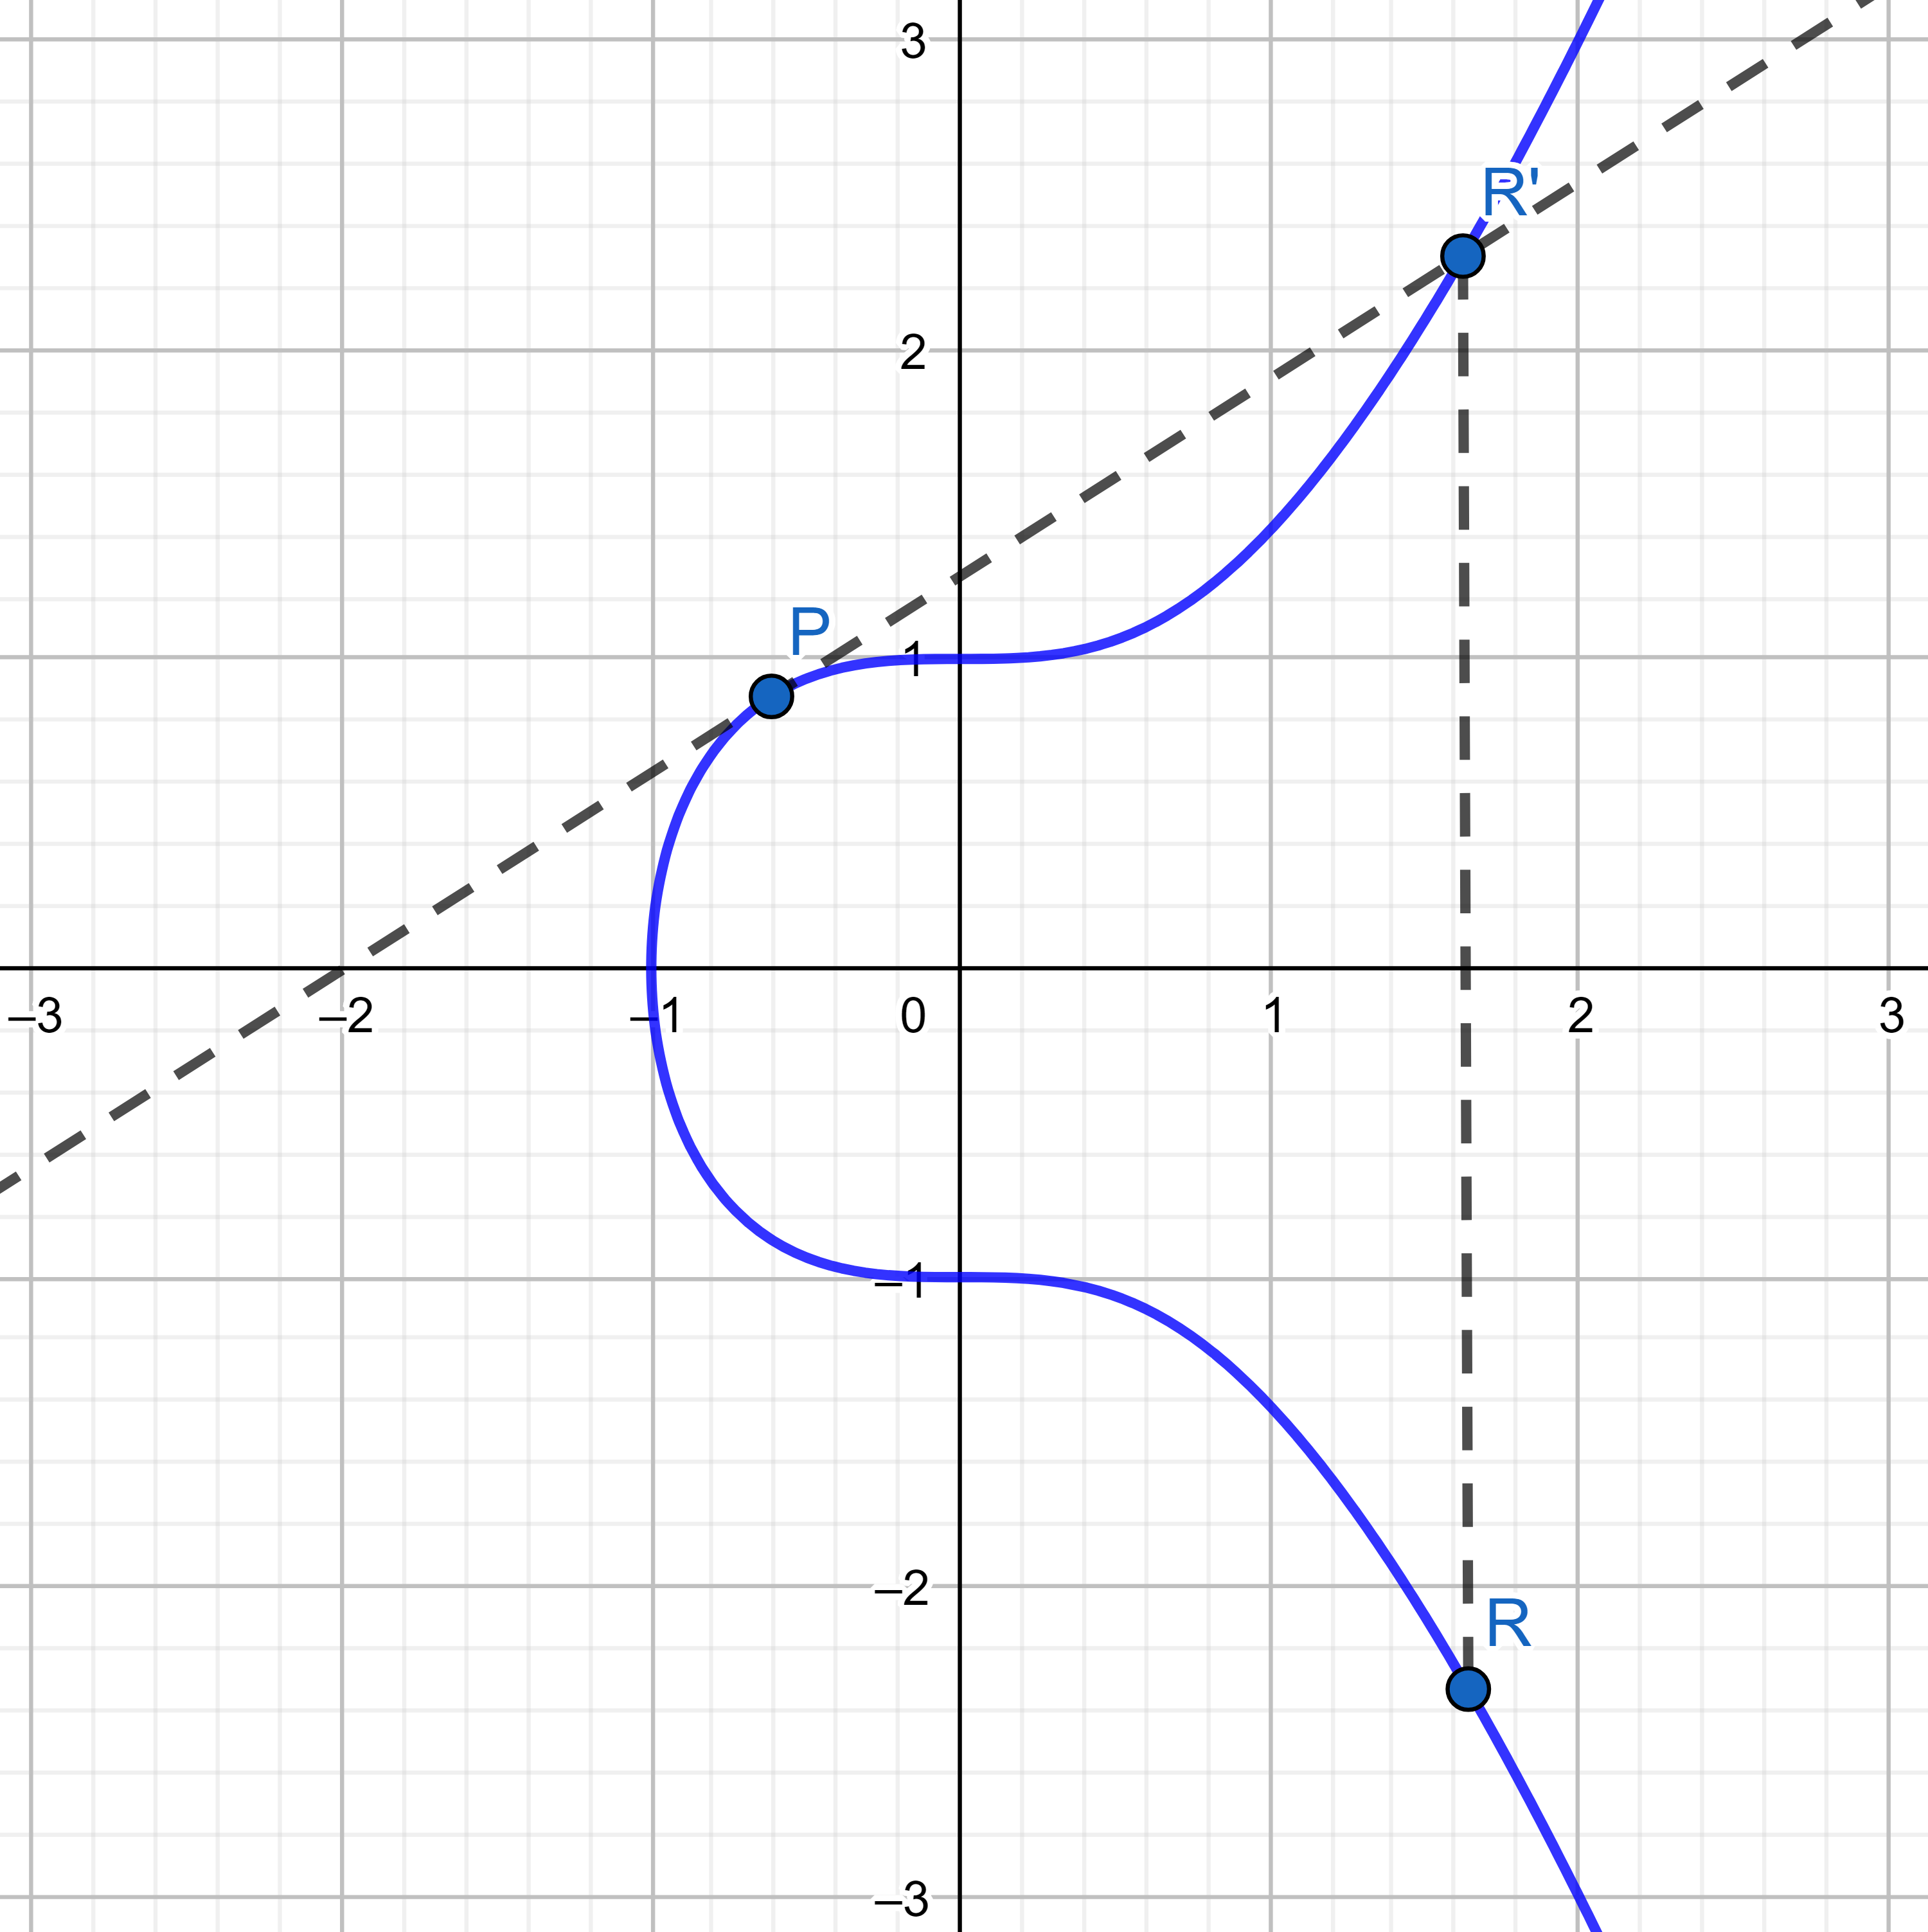
\includegraphics[width=.9\textwidth]{02-elliptikus-gorbe-kriptografia/elliptikus-gorbe-osszeadas2.png}
        \caption{Elliptikus görbe pontjának összeadása önmagával.}
        \label{Figure::ECC::EllipticCurveAddition2}
    \end{subfigure}
\end{figure}


\subsubsection{Az $E(K) : y^2 = x^3 + ax + b$ görbe tulajdonságai \protect\footnote{Ha $K$ karakterisztikája nem $2$.}}

\begin{outdentlist}
    \item[]
    \textbf{Egységelem.} $P + O = O + P = P$, minden $P \in E(K)$ esetén.

    \item[]
    \textbf{Ellentettek.} Ha $P = (x, y) \in E(K)$, akkor $(x, y) + (x, -y) = O$. Az $(x, -y)$ pontot $-P$-vel jelöljük és $P$ ellentettjének nevezzük. $-P$ is $E(K)$ egy pontja.

    \item[]
    \textbf{Pontok összeadása.} Legyen $P = (x_1, y_1) \in E(K)$ és $Q = (x_2, y_2) \in E(K)$, úgy hogy $P \neq \pm Q$. Ekkor $P + Q = (x_3, y_3)$, ahol 
    \begin{center}$x_3 = \big(\frac{y_2 - y_1}{x_2 - x_1}\big)^2 - x_1 - x_2$ és $y_3 = \frac{y_2 - y_1}{x_2 - x_1}(x_1 - x_3) - y_1$.\end{center}

    \item[]
    \textbf{Pont duplázás.} Legyen $P = (x_1, y_1) \in E(K)$, úgy hogy $P \neq -P$. Ekkor $2P = (x_3, y_3)$, ahol
    \begin{center}$x_3 = \big(\frac{3x_1^2 + a}{2y_1}\big)^2 - 2x_1$ és $y_3 = \frac{3x_1^2 + a}{2y_1}(x_1 - x_3) - y_1$.\end{center} Ha $P = -P$, akkor $2P = O$.
\end{outdentlist}

\subsection{Pontok skalár szorzása}

Az elliptikus görbe pontjait tetszőleges $k$ skalárral megszorozhatjuk, ami annyit jelent, hogy a pont $k$ példányát összeadjuk. Tehát ezen szorzás kiszámításának triviális módja az, ha elvégzünk $k - 1$ darab összeadást, azonban ez nagy $k$ esetén egy nagyon költséges lépéssorozat. Ezzel szemben létezik néhány kevésbé egyszerű, de sokkal hatékonyabb algoritmus is a szorzás elvégzésére.

\subsubsection{Double-and-Add}

A Horner séma \cite{Horner::HornerScheme} vagy \textit{Double-and-Add} nevű módszer egy hatékony megoldást nyújt elliptikus görbe pontjának skaláris szorzására, hasonlóan polinomok Horner-elrendezéséhez: Legyen a $k$ bináris felírása $\sum\limits_{i = 0}^{t-1} k_i 2^i$, ekkor $$kP = \sum_{i = 0}^{t-1} k_i 2^i(P) = k_0P + 2(k_1P + 2(k_2P + 2(... + 2(k_{t-1}P)...))).$$

A fenti képlet pszeudokódját az Algoritmus \dotref{algorithm:doubleAndAdd} jeleníti meg.
\begin{algorithm}[H]
    \floatname{algorithm}{Algoritmus}
    \caption{Double-and-Add algoritmus}
    \label{algorithm:doubleAndAdd}
    \begin{algorithmic}
        \Procedure{ScalarMultiply}{$k, P$} \Comment{$k=(k_{t-1},...,k_1,k_0)_2,P \in E(\mathbb{F}_q).$}
        \State $Q \gets O$
        \For {$i \gets t - 1$ downto $0$}
            \State {$Q \gets 2Q$}
            \If {$k_i = 1$} 
                \State $Q \gets Q + P$
            \EndIf
        \EndFor
        \State \Return {$Q$}
        \EndProcedure
    \end{algorithmic}
\end{algorithm}

Ezen felül számos lehetőség van optimalizálásra, mint például újabb, gyorsabb algoritmusok használata, azonban a dolgozat szemponjából ezek nem fontosak.

\section{Elliptikus görbék a kriptográfiában}

A kriptográfiában olyan elliptikus görbéket szokás alkalmazni, amelyek véges test felett vannak definiálva. A megelőzőleg bevezetett műveletek ekkor is érvényesek, az
eredmény pedig mindig a görbe egy pontja lesz. Elterjedtek az $\mathbb{F}_p$ felett értelmezett görbék, ahol $p$ egy prímszám. Ekkor a pontok koordinátáival mindig modulo $p$ kell számolni.

Az elliptikus görbén alapuló kriptográfiai sémák biztonságosságát az elliptikus diszkrét logaritmus probléma nehézsége adja.

\begin{definition*}
Az \textbf{elliptikus diszkrét logaritmus probléma} (ECDLP): Adott egy $E$ elliptikus görbe az $\mathbb{F}_q$ véges test felett, egy $n$ rendű $P \in E(\mathbb{F}_q)$ pont, valamint egy $Q$ pont, amely $P$ többszöröse. Keressük azt az $l \in [0, n - 1]$ egész számot, amelyre $Q = lP$ teljesül. Ezt a számot a $Q$ pont $P$ alapú elliptikus diszkrét logaritmusának nevezzük.
\end{definition*}

A definícióban bevezetett diszkrét logaritmus meghatározására nem ismert hatékony algoritmus.

\subsection{Miért válasszuk az elliptikus görbe kriptográfiát?}

Napjainkban az egyik legelterjedtebb aszimmetrikus titkosítási módszer az RSA algoritmus, ami a biztonságosságát a faktorizáció problémájából nyeri. Az RSA matematikai háttere sokkal egyszerűbbnek mondható, mint az elliptikus görbéken alapuló algoritmusoké, ezért implementálása sokkal egyszerűbb.

A faktorizáció ugyanakkor kevésbé nehéz probléma, mint az elliptikus diszkrét logaritmus probléma. Ahhoz, hogy az RSA algoritmus elérje a kellő biztonságosságot, sokkal nagyobb bithosszúságú kulcsokkal kell dolgoznia, mint az elliptikus görbéken alapuló algoritmusoknak \cite{Miller::ECC}. Ahogy a NIST ajánlásából olvasható, 160-521 bithosszúságú kulcs megfelelő az elliptikus görbén alapuló algoritmusok esetén \cite{NIST::EllipticCurve}, ezzel szemben az RSA esetén sokkal hosszabb, 1024-15360 bithosszúságú kulcsok szükségesek. Az NSA táblázat formájában is összevetette a NIST ajánlásait a különböző méretű AES kulcsok titkosításához szükséges RSA és elliptikus görbe kulcshosszakról \cite{NSA::EllipticCurve}.

A nagy kulcsok lassítják a számítást, ezért úgy gondoljuk, hosszú távon az elliptikus görbén alapuló algoritmusok jobban skálázhatók, mint az RSA.

\subsection{Elliptikus görbe könyvtárak}

Munkánk során több különböző elliptikus görbe aritmetikát megvalósító könyvtárat is megvizsgáltunk, amelyeket a \dotref{table::ECLibs} táblázat foglal össze.
\begin{table}[H]
    \centering
    \begin{tabular}{|l|l|l|}
        \hline
        \multicolumn{1}{|c|}{\textbf{Könyvtár neve}} & \multicolumn{1}{c|}{\textbf{Link}} & \multicolumn{1}{c|}{\textbf{Licenc}} \\ \hline
        libecc                                       & \url{https://github.com/ANSSI-FR/libecc} & BSD és GPL v2                         \\ \hline
        MIRACL                                       & \url{https://github.com/miracl/MIRACL}   & GNU AGPL v3                           \\ \hline
        PARI                                         & \url{https://pari.math.u-bordeaux.fr/}   & GNU GPL                               \\ \hline
        SageMath                                     & \url{http://www.sagemath.org/}           & GNU GPL                               \\ \hline
        snowshoe                                     & \url{https://github.com/catid/snowshoe}  & BSD 3-Clause                          \\ \hline
    \end{tabular}
    \caption{Elliptikus görbe aritmetikát megvalósító könyvtárak.}
    \label{table::ECLibs}
\end{table}
A libecc és a snowshoe dokumentációját elégtelennek találtuk, ami rendkívül megnehezítette volna a felhasználásukat.

A SageMath bár jól dokumentált, azonban egy óriási méretű könyvtár, melynek csak néhány elemére lett volna szükségünk. 

A PARI \cite{PARI} és a MIRACL között a döntést hozó tényező az volt, hogy a PARI fejlesztőit a témavezetőnk útján közelebbről is ismerjük.

Később azonban a fejlesztés során kellett rájönnünk, hogy céljaink elérése érdekében saját elliptikus görbe aritmetikát kell implementálnunk. 

Az egyik indok, ami erre a döntésre juttatott minket, hogy böngészőben kliensoldalon, akár mobil eszközökről is használhatóvá akartuk tenni a CryptID-nek nevezett könyvtárunkat, ami megköveteli a kis méretet az internetes adatforgalom csökkentése érdekében. A vizsgált elliptikus görbe műveleteket megvalósító könyvtárak számos olyan funkciót is tartalmaznak, amikre nekünk nem volt szükségünk, ezzel fölösleges mérettöbletet alkotva.

Másik fontos szempontunk az volt, hogy a saját implementációval úgy gondoljuk, leegyszerűsítettük a jövőbeli optimalizációs és kutatási tevékenységeink folytatását ezen a területen.

    \chapter{Identity-based Encryption}

Az Identity-based Encryption olyan nyilvános kulcsú titkosítási eljárás, amely esetén a publikus kulcs egy tetszőleges karaktersorozat lehet, amely egyértelműen azonosítani tud egy entitást.

A fejezetben kifejtjük az IBE célját és működését, azonban ezt megelőzően még egy rövid betekintést adunk a párosítások működésébe és fontosságába.

\section{Párosítás-alapú kriptográfia}

A párosítás lényege, hogy egy bizonyos csoporton definiált nehéz probléma átalakítható egy könnyebb problémává egy másik csoport felett. Ez a leképezés számos új kriptográfiai séma létrejöttét tette lehetővé, köztük az Identity-based Encryptionét.

\subsection{A párosítás elterjedése a kriptográfiában}

A párosítás-alapú kriptográfia egy nagyon fiatal terület, mely a párosítások kriptoanalízisben való alkalmazásából fejlődött ki \cite{ReducingEllipticCurveLogarithms}. A MOV redukcióval sikerült szuperszinguláris görbék esetén az elliptikus görbe diszkrét logaritmus problémát redukálni egy véges testen értelmezett diszkrét logaritmus problémává.

A következő lépéseket a párosítás-alapú kriptográfia kialakulása felé Joux tette, aki a Weil és Tate párosításokat használta a Diffie-Hellmann protokoll egy variációjának létrehozására \citeyear{JouxPairingBasedCrypto}.

Ezt követően készítette el Boneh és Franklin a csoportok közti bilineáris leképezésen (például Weil és Tate párosításon) alapuló IBE rendszerüket \citeyear{Boneh::IdentityBasedEncryptionFromTheWeilPairing}. 

Ezeket a munkákat tekinthetjük a párosítás-alapú kriptográfia úttörőinek.

\subsection{A párosítás tulajdonságai}

Az alfejezetben El Mrabet és Joye munkáját vesszük alapul a párosítás tulajdonságainak ismertetéséhez \citeyear{GuideToPairingBasedCrypto}.

Jelöljön $G_1, G_2$ additív, míg $G_\mathbb{T}$ multiplikatív $r$ rendű csoportokat. Az $e$ párosítás egy olyan $e : G_1 \times G_2 \rightarrow G_\mathbb{T}$ leképezés, amely a következő tulajdonágokkal rendelkezik:
\begin{outdentlist}
    \item[] \textbf{Bilineáris.} Jelölje $\mathbb{Z}_r$ az egész számok halmazát modulo $r$, ekkor $\forall P_1 \in G_1, P_2 \in G_2$ és $a, b \in \mathbb{Z}_r$ esetén $e(aP_1, bP_2) = e(P_1, P_2)^{ab}$.

    \item[] \textbf{Nem elfajuló.} Ha $P_1 \neq 0_{G_1}$ és $P_2 \neq 0_{G_2}$, akkor $e(P_1, P_2) \neq 1_{G_\mathbb{T}}$, ahol $0_{G_1}$ (illetve $0_{G_2}$ és $1_{G_\mathbb{T}}$) az egységeleme a $G_1$ csoportnak (illetve $G_2$ és $G_\mathbb{T}$ csoportnak).

    \item[] \textbf{Hatékonyan számítható.}

    \item[] \textbf{Nehezen megfordítható.}
\end{outdentlist}

A kriptográfiában elterjedten használt párosítási módszerek a Weil és a Tate párosítás.

\section{Személyre szabott titkosítás}

Ahogy azt a fejezet elején említettük, az IBE egy olyan nyilvános kulcsú titkosítási eljárás, melynek esetén a publikus kulcs tetszőleges olyan karaktersorozat lehet, amely egyértelműen azonosítani tud egy entitást. Fontos azonban, hogy nemcsak az azonosító, hanem az annak hatókörét jelentő domain is tetszőleges. Lehet csupán néhány fős (például egy vállalat), vagy akár globális kiterjedésű is.

A kitalált séma célja az volt, hogy az entitások kulcscsere nélkül tudjanak egymásnak titkosított üzenetet küldeni \cite{AdiShamirIBE}. Azonban éveken át sikertelenül próbáltak létrehozni jól működő IBE sémákat.

A már említett, Boneh és Franklin \citeyear{Boneh::IdentityBasedEncryptionFromTheWeilPairing} nevéhez fűződő rendszer volt az első, amely teljesen működőképesnek és a gyakorlatban is hatékonyan használhatónak bizonyult.

\subsection{Boneh-Franklin Identity-based Encryption}

Shamir eredeti elképzelése az volt, hogy a publikus kulcsa mindenkinek az email címe legyen. Ennek köszönhetően megspórolhatóvá válna a publikus kulcs megszerzésének költsége.

Az elgondolt séma működése egyszerű. Mikor Kriszta titkosított emailt szeretne küldeni Aladárnak, egyszerűen titkosítja azt Aladár email címével, majd elküldi. Ahhoz, hogy Aladár az üzenetet el tudja olvasni, előbb vissza kell fejtenie. Ezt úgy tudja megtenni, hogy a használt alkalmazás által specifikált módon azonosítja magát, ami után eléri a privát kulcs generátort (PKG). A PKG felelős a felhasználók privát kulcsának elkészítéséért. Az elkészült privát kulcs eljut Aladárhoz, aki azt felhasználva vissza tudja fejteni az üzenetet. Ez a folyamat megtekinthető a \dotref{Figure::ShamirIBE} ábrán.

\begin{figure}[H]
    \centering
    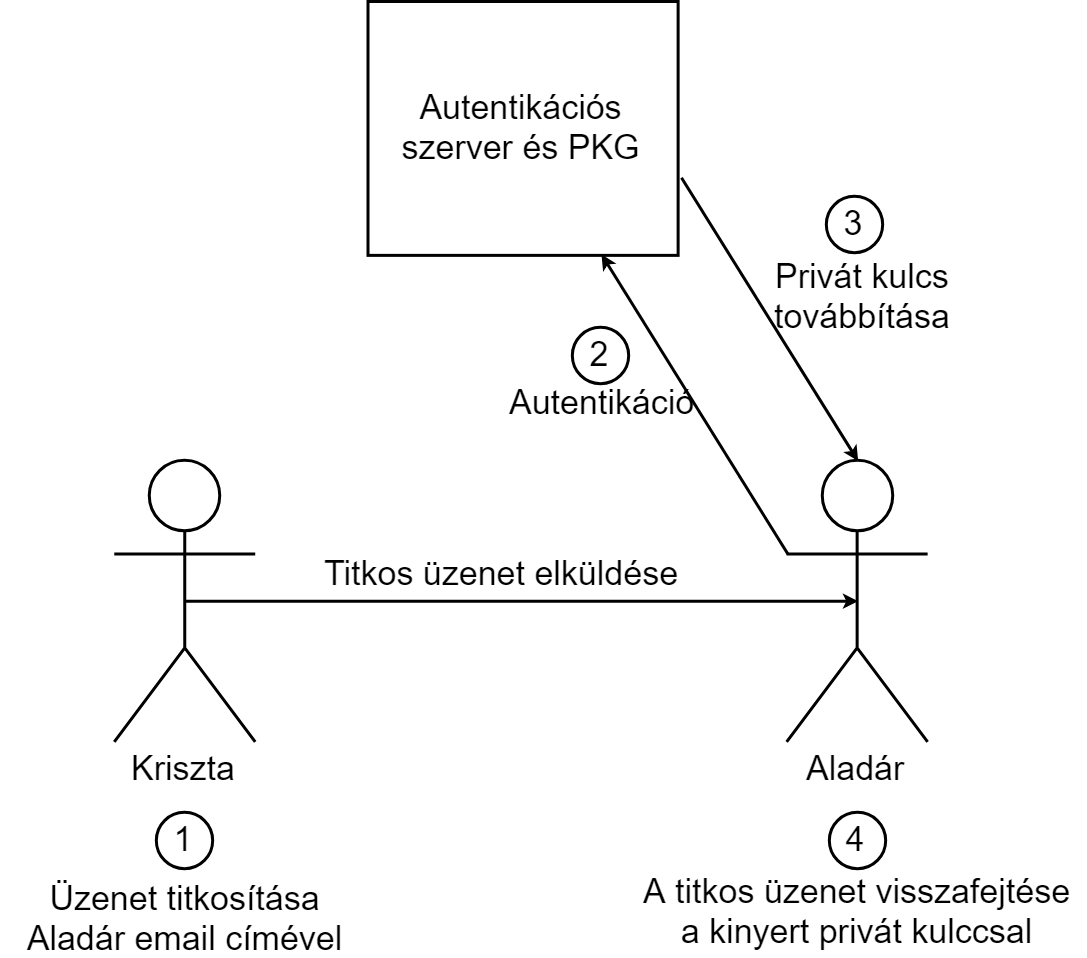
\includegraphics[width=0.6\textwidth]{03-identity-based-encryption/IBE.png}
    \caption{Az IBE működése.}
    \label{Figure::ShamirIBE}
\end{figure}

A séma előbb vázolt működéséhez szükséges még egy, az ábrán nem szereplő előkészítő lépés is. Ennek részeként létrejönnek az úgynevezett publikus paraméterek, valamint a mesterkulcs. Ahhoz, hogy titkosított kommunikációt folytathassunk, először be kell szereznünk a publikus paramétereket; kiemelendő ugyanakkor, hogy erre csak egyszer van szükség, hiszen ezek a paraméterek függetlenek mind a feladótól, mind a címzettől. Míg a publikus paraméterek a rendszer összes felhasználója számára ismertek, addig a mesterkulccsal csupán a PKG rendelkezik  – a privát kulcsok előállítása ugyanis csak ennek birtokában lehetséges.

Boneh és Franklin egy ennek az elképzelésnek eleget tevő rendszert dolgozott ki, amelyet négy algoritmus alkot. Ezek leírásához Martin könyvét \citeyear{Martin::IntroductionToIdentityBasedEncryption} és Kovács diplomamunkáját \citeyear{Kovacs::IBE} vettük alapul.

Az egyes algoritmusok ismertetésének és az azokat követő pszeudokódoknak a megértését elősegíti a \dotref{table::IBEParams} táblázat, amiben összefoglaltuk a különböző paraméterek jelentését.

\begin{table}[H]
    \centering
    \begin{tabular}{|l|l|l|}
        \hline
        \multicolumn{1}{|c|}{\textbf{Paraméter neve}} & \multicolumn{1}{c|}{\textbf{Típusa}} & \multicolumn{1}{c|}{\textbf{Megjegyzés}}              \\ \hline
        $q$                                                  & prím                                 & \multicolumn{1}{c|}{-}                                        \\ \hline
        $p$                                                  & prím                                 & \multicolumn{1}{c|}{-}                                        \\ \hline
        $E(\mathbb{F}_p)$                                     & elliptikus görbe                     & \multicolumn{1}{c|}{-}                                        \\ \hline
        $G_1$                                                & az $E(\mathbb{F}_p)$ ciklikus részcsoportja                     & generátora $P$            \\ \hline
        $G_\mathbb{T}$                                                & az $E(\mathbb{F}_p)$ ciklikus részcsoportja                     & generátora $e(P, P)$        \\ \hline
        $e$                                                  & párosítás                            & $e : G_1 \times G_1 \rightarrow G_\mathbb{T}$                          \\ \hline
        $n$                                                  & egész szám                           & a titkosítatlan szöveg hossza                                 \\ \hline
        $P$                                                  & elliptikus görbe pontja              & $P \in E(\mathbb{F}_p)$                                        \\ \hline
        $sP$                                                 & elliptikus görbe pontja              & $sP \in E(\mathbb{F}_p)$                  \\ \hline
        $H_1$                                                & kriptográfiai hash függvény          & $H_1 : \{0, 1\}^* \rightarrow G_1$                            \\ \hline
        $H_2$                                                & kriptográfiai hash függvény          & $H_2 : G_\mathbb{T} \rightarrow \{0, 1\}^n$                            \\ \hline
        $H_3$                                                & kriptográfiai hash függvény          & $H_3 : \{0, 1\}^n \times \{0, 1\}^n \rightarrow \mathbb{Z}_q$ \\ \hline
        $H_4$                                                & kriptográfiai hash függvény          & $H_4 : \{0, 1\}^n \rightarrow \{0, 1\}^n$                     \\ \hline
    \end{tabular}
    \caption{A Boneh-Franklin Identity-based Encryption paraméterei.}
    \label{table::IBEParams}
\end{table}

\begin{outdentlist}
    \item[]\textbf{Setup.}
    Ez a függvény felelős a rendszer inicializálásáért, a felhasználóhoz tartozó publikus paraméterek és a mesterkulcs előállításáért. Bemenetként a biztonsági fokot meghatározó $k$ paramétert várja. A \dotref{table::RFC::SecurityParam} táblázatban az RFC 5091 ajánlásai láthatók a különböző $k$ értékekre vonatkozóan \cite{RFC5091}. A táblázatban szereplő $k$ értékek a hasonló biztonságot nyújtó RSA kulcshosszak méretét jelképezik, ahogy azt az NSA táblázatából is leolvashatjuk \cite{NSA::EllipticCurve}.

    \begin{table}[H]
        \centering
        \begin{tabular}{|l|l|l|l|}
            \hline
            \multicolumn{1}{|c|}{\textbf{$k$ értéke}} & \multicolumn{1}{c|}{\textbf{$q$ bithosszúsága}} & \multicolumn{1}{c|}{\textbf{$p$ bithosszúsága}} & \multicolumn{1}{c|}{\textbf{Jelölése a dolgozatban}}\\ \hline
            $1024$                           & $160$                                  & $512$                           & LOWEST                                  \\ \hline
            $2048$                           & $224$                                  & $1024$                           & LOW                                 \\ \hline
            $3072$                           & $256$                                  & $1536$                           & MEDIUM                                 \\ \hline
            $7680$                           & $384$                                  & $3840$                           & HIGH                                 \\ \hline
            $15360$                          & $512$                                  & $7680$                           & HIGHEST                                 \\ \hline
        \end{tabular}
        \caption{Az RFC 5091 ajánlásai a biztonsági paraméternek megfelelő bithosszakra.}
        \label{table::RFC::SecurityParam}
    \end{table}

    A \textit{Setup} pszeudokóját az Algoritmus \ref{algorithm:setup} adja meg.

    \begin{algorithm}[H]
        \floatname{algorithm}{Algoritmus}
        \caption{Setup}
        \label{algorithm:setup}
        \begin{algorithmic}
            \Procedure{Setup}{$k$} 
            \State $q$ prím inicializálása \Comment $k$ paraméternek megfelelően
            \State $p$ prím inicializálása \Comment $k$ paraméternek megfelelően
            \State $E(\mathbb{F}_p)$ elliptikus görbe inicializálása
            \State $P = randomPoint(E(\mathbb{F}_p))$ \Comment $P \in E(\mathbb{F}_p)$
            \State $G_1$ csoport generátora legyen $P$
            \State $e : G_1 \times G_1 \rightarrow G_\mathbb{T}$ párosítás kiválasztása
            \State $G_\mathbb{T}$ csoport generátora legyen $e(P, P)$
            \State $s = randomInteger(q)$ \Comment $s \in \mathbb{Z}_q$
            \State $H_1 : \{0, 1\}^* \rightarrow G_1$ kriptográfiai hash függvény kiválasztása
            \State $H_2 : G_\mathbb{T} \rightarrow \{0, 1\}^n$ kriptográfiai hash függvény kiválasztása
            \State $H_3 : \{0, 1\}^n \times \{0, 1\}^n \rightarrow \mathbb{Z}_q$ kriptográfiai hash függvény kiválasztása
            \State $H_4 : \{0, 1\}^n \rightarrow \{0, 1\}^n$ kriptográfiai hash függvény kiválasztása
            \State $PublicParameters = (G_1, G_\mathbb{T}, e, n, P, sP, H_1, H_2, H_3, H_4)$
            \State \Return $s, PublicParameters$ \Comment $s$ a mesterkulcs
            \EndProcedure
        \end{algorithmic}
    \end{algorithm}

    \item[]\textbf{Extract.}
    Az azonosítóhoz tartozó privát kulcs kinyerésére szolgáló függvény. Bemenetként egy $ID$ azonosítót vár. A privát kulcsot csak egyszer kell generálni, aztán mindaddig használható, amíg nem kompromittálódik. Ha egy privát kulcs kompromittálódik, például ellopják, az azt jelenti, hogy minden üzenet, ami az ahhoz tartozó nyilvános paraméterekkel lett titkosítva, veszélyben van. A séma nem ad támogatást ilyen veszéllyel szemben, azonban a \textit{Setup} függvény újrafuttatásával új nyilvános paraméterek generálhatók, ekképpen az új üzenetek ismét biztonságban lehetnek.
    \begin{algorithm}[H]
        \floatname{algorithm}{Algoritmus}
        \caption{Extract}
        \label{algorithm:extract}
        \begin{algorithmic}
            \Procedure{Extract}{$ID$} 
            \State $Q_{ID} = H_1(ID)$
            \State \Return $sQ_{ID}$
            \EndProcedure
        \end{algorithmic}
    \end{algorithm}

    \item[]\textbf{Encrypt.}
    Az üzenet titkosítását végző függvény. Bemenetként egy $M$ üzenetet és egy $ID$ azonosítót vár.
    \begin{algorithm}[H]
        \floatname{algorithm}{Algoritmus}
        \caption{Encrypt}
        \label{algorithm:encrypt}
        \begin{algorithmic}
            \Procedure{Encrypt}{$M, ID$} 
            \State $Q_{ID} \gets H_1(ID)$
            \State $\sigma \gets randomBits(n)$ \Comment $\sigma \in \{0, 1\}^n$
            \State $r \gets H_3(\sigma, M)$
            \State $C_1 \gets rP$
            \State $C_2 \gets \sigma \oplus H_2(e(rQ_{ID}, sP))$
            \State $C_3 \gets M \oplus H_4(\sigma)$
            \State $C \gets (C_1, C_2, C_3)$
            \State \Return {$C$}
            \EndProcedure
        \end{algorithmic}
    \end{algorithm}

    \item[]\textbf{Decrypt.}
    A titkos üzenet visszafejtéséért felelős függvény. Bemenetként egy $C$ titkos üzenetet és egy $sQ_{ID}$ privát kulcsot vár.
    \begin{algorithm}[H]
        \floatname{algorithm}{Algoritmus}
        \caption{Decrypt}
        \label{algorithm:decrypt}
        \begin{algorithmic}
            \Procedure{Decrypt}{$C, sQ_{ID}$} 
            \State $\sigma \gets C_2 \oplus H_2(e(sQ_{ID}, C_1))$
            \State $M \gets C_3 \oplus H_4(\sigma)$
            \State $r = H_3(\sigma, M)$
            \If {$C_1 \neq rP$} 
                \State \Return {error} \Comment Hibás bemenet.
            \EndIf
            \State \Return {$M$}
            \EndProcedure
        \end{algorithmic}
    \end{algorithm}
\end{outdentlist}

Fontos megjegyezni, hogy az \textit{Encrypt} és \textit{Decrypt} függvények egymás inverzét alkotják. Ez azt jelenti, hogy ha $\mathcal{M}$ jelöli az üzenetteret, akkor $\forall M \in \mathcal{M} :$ \textit{Decrypt}(\textit{Encrypt}($M$, $ID$), $sQ_{ID}$) $= M$ \cite{Boneh::IdentityBasedEncryptionFromTheWeilPairing}.

A bizonyítás a párosítás alapvető tulajdonságát használja ki, mely szerint:
$$e(rQ_{ID},sP)=e(Q_{ID},P)^{rs}=e(sQ_{ID},rP).$$

    \chapter{WebAssembly}

Míg a megelőző fejezetek a dolgozat eredményét jelentő könyvtár kriptográfiai alapjait fektették le, addig ebben a fejezetben az implementációhoz használt egyik legfontosabb technológiát, a WebAssemblyt (röviden: Wasm) mutatjuk be részletesen. 

Annak érdekében, hogy érezhető legyen a WebAssembly valódi jelentősége, ismertetésre kerülnek a hasonló célokat szolgáló, azonban ma már túlhaladottnak tekinthető eszközök. Ezt követően a WebAssembly áttekintését adjuk, kiemelt figyelmet szentelve azoknak az előnyös tulajdonságoknak, melyek megkülönböztetik a korábbi technológiáktól. Végül egy rövid példa zárja a fejezetet, ízelítőt adva a fejlesztési folyamatból.

\section{Előzmények}

A dinamikus weboldalak létrehozását lehetővé tevő JavaScript programozási nyelv 1995-ben jelent meg először a Netscape Navigator 2.0 böngészőben \cite{JavaScriptAnnouncement}. Bár szerveroldali alkalmazása már a kezdetektől is lehetséges volt, azonban a 2010-es évekig (a Node.js feltűnéséig) inkább a kliensoldalon játszott meghatározó szerepet, hiszen az első pillanattól kezdve támogatta a HTML oldalak manipulációját, miközben egyszerű, laikusok számára is érthető szintaxissal bírt.

Ugyanakkor nem a JavaScript az egyetlen olyan technológia, mely az elmúlt évtizedekben a dinamikus webes tartalmak elkészítését, vagy egyszerűen csak a böngészőben való, lehetőleg hatékony kódfuttatás elősegítését szolgálta. A teljesség igénye nélkül érdemes megemlékezni a következő technológiákról, melyek mindegyike ilyen, vagy olyan szempontból, de az előbbi célokra készült, így egyúttal a WebAssembly előzményének is tekinthető:

\begin{itemize}
    \item
    Java Applet,

    \item
    Adobe Flash,

    \item
    ActiveX,

    \item
    Native Client (NaCl), illetve Portable Native Client (PNaCl),

    \item
    asm.js.
\end{itemize}

A következőkben e technológiák főbb jellemzőit tekintjük át: az előbbi három esetében csak érintőlegesen, míg a (P)NaCl és az asm.js esetében részletesebben.

\subsection{Korai beépülő modulok}

A Java programozási nyelvhez kapcsolódó platformfüggetlen infrastruktúrát használják ki az \textit{appletek}, melyek más alkalmazásokba beágyazható kis programok\cite{JavaDocs::java.applet.Applet}. Az egyik legnépszerűbb beágyazó környezetet a webböngészők jelentik, melyek beépülő modulok segítségével képesek az \textit{appletek} megjelenítésére \cite{JavaPlugInTechnology}. Természetesen az \textit{appletek} forráskódja a beágyazó böngészőtől teljesen független. Kiemelendő, hogy az \textit{appletek} alapértelmezés szerint egy zárt, úgynevezett \textit{sandbox} környezetben futnak, mely megakadályozza, hogy kártékony tevékenységeket hajtsanak végre a felhasználó tudta nélkül \cite{TheJavaTutorials::JavaApplets}.

A Flash először csak gyors rajzolási és animációs képességekkel kívánta felruházni a böngészőket, az évek során azonban egy átfogó multimédia platformmá fejlődött \cite{Gay::TheHistoryOfFlash}. Létrejöttében kulcsszerepet játszott az \textit{appletek} multimédiás célokra történő alkalmatlansága. A Flash animációk böngészőben történő megjelenítéséhez szintén egy beépülő modul szükséges, ez a Flash Player \cite{AdobeFlashPlayer}.

Említésre méltó a Microsofthoz köthető ActiveX Technologies keretrendszer, mely úgynevezett ActiveX Controlok útján tette lehetővé dinamikus komponensek és objektumok beágyazását a HTML oldalakba \cite{MicrosoftAnnouncesActiveXTechnologies}. Habár az ActiveX Controlok is egy beépülő böngésző modult igényelnek a megfelelő működéshez, azonban a technológia jelentősen eltér az előzőleg látottaktól. Egyfelől az egyes komponensek platformfüggő binárisok formájában kerülnek terjesztésre \cite{Grimes::MaliciousMobileCode}, másfelől azok közvetlenül kerülnek lefuttatásra, így tetszőleges műveleteket végrehajthatnak a felhasználó számítógépén \cite{DesigningSecureActiveXControls}.

Ma már ezen három technológia mindegyike túlhaladottnak tekinthető. Az Applet API a Java 9-ben már \textit{deprecated} annotációval bír \cite{JEP289::DeprecateTheAppletAPI}, a Flash támogatását az Adobe 2020-ban végleg beszünteti \cite{FlashAndTheFutureOfInteractiveContent}, az ActiveX pedig az úgynevezett \textit{evergreen} böngészők egyikében sem támogatott már, még a Microsoft Edge-ben sem \cite{ABreakFromThePast}.

\subsection{Native Client, Portable Native Client}

Míg az előzőleg felsorolt technológiák inkább a böngésző, mint alkalmazásfejlesztési platform hiányosságait kívánták pótolni, addig a Google ernyője alatt megszülető Native Client (röviden NaCl) a teljesítményre fókuszál. A NaCl a natív (azaz például C vagy C++ nyelven írt) programok hatékony futtatását tette lehetővé a böngésző által biztosított \textit{sandbox} környezetben \cite{Yee::NativeClient}. A NaCl platformfüggetlen testvére a Portable Native Client (röviden PNaCl), mely a HTML oldalakba való beágyazást is biztosítja \cite{NativeClient::NaClAndPNaCl}.

A PNaCl modulokat (\textit{pexe}) egy LLVM-alapú fordító segítségével lehet előállítani. Érdekesség, hogy az így elkészült modul a fordító belső, átmeneti reprezentációját használja, a tartalmazott kód ugyanis LLVM IR (\textit{intermediate representation}) nyelvű. A létrejött modulok végrehajtása két lépésből áll. Először a böngészőbe épített \textit{ahead-of-time} (AOT) fordító platformfüggő kódot készít, majd pedig a NaCl modulok futtatásához is használt \textit{sandbox} ténylegesen lefuttatja a kódot \cite{NativeClient::TechnicalOverview}.

Noha a PNaCl valóban alkalmas volt a böngészőn belüli gyors és biztonságos végrehajtásra, a Google Chrome-on kívül sosem terjedt el igazán. Ma már a Google is inkább a WebAssembly használatát javasolja \cite{Nelson::GoodbyePNaClHelloWebAssembly}.

\subsection{asm.js}

Az egyetlen programozási nyelv, mely stabilan elérhető az összes platform összes böngészőjében, a JavaScript. Ezen felismerésre alapozva kialaultak olyan eszközök, melyek valamilyen másik programozási nyelv kódbázisát fordítják a böngészőben futtatható \mbox{JavaScriptre} \cite{ListOfLanguagesThatCompileToJS}. Ezek közül is kiemelkedik az asm.js, mely a böngészőben történő nagyteljesítményű kódvégrehajtást helyezi előtérbe.

A futási sebesség növekedése két tényező eredménye. Egyfelől a fordítás első lépése az LLVM infrastruktúrán keresztül valósul meg, mely eleve egy optimalizált átmeneti reprezentációt állít elő. Ezt az Emscripten a JavaScript egy rendkívül szűk részhalmazára fordítja, mely a hatékonyság mögötti második faktor. Ez a részhalmaz ugyanis a \mbox{JavaScript} dinamikus jellemzőit elhagyja, így a fokozatosan optimalizáló \textit{just-in-time} (JIT) fordító helyett a kód fordításához rögtön egy, a böngésző teljes optimalizálási eszközkészletét kihasználó AOT fordító használható \cite{Zakai::BigWebAppCompileIt}. Kiemelendő azonban, hogy az asm.js alkalmazása akkor is sebességnövekedéssel jár, ha a böngésző csak JIT-et használ.

Habár az asm.js nem tekinthető elavultnak, a WebAssembly elterjedésével párhuzamosan jelentősége várhatóan csökkenni fog. Az Emscripten például alapértelmezés szerint már WebAssembly kódot állít elő asm.js helyett \cite{GitHub::EmitWebAssemblyByDefaultInsteadOfAsmJs}.

\section{A WebAssembly, mint modern célplatform}

A megelőző pontok azon technológiák közül szemezgettek, melyek a '90-es évek közepétől kezdődően a web, mint alkalmazásfejlesztési platform gazdagítását, felgyorsítását szolgálták. Szerepük a böngészők (és a web) fejlődésében vitathatatlan, hiszen a ma ismert szabványos és modern Web API-k funkcionalitását nyújtották, jóval azok megjelenése előtt. Ugyanakkor a megfelelő W3C szabványok feltűnésével és elterjedésével ezek a bővítmények szükségtelenné, mi több, a fejlődés akadályozóivá váltak.

A multimédiás lehetőségeket biztosító bővítmények (például: Flash, Shockwave, Silverlight, ActiveX) visszaszorulásában többek között a HTML5, a CSS3, az SVG, és a WebGL játszott fontos szerepet. A hatékony, natívhoz mérhető sebességű kódvégrehajtásra pedig a WebAssembly nyújt az egyes platformokon és böngészőkön átívelő modern, egységes megoldást.

\subsection{A WebAssembly specifikáció}

A WebAssembly a W3C WebAssembly Community Group által 2015-től fejlesztett virtuális ISA (\textit{instruction set architecture}), melynek elsődleges célja a weben történő nagysebességű kódvégrehajtás, ugyanakkor tetszőleges környezetbe beágyazható \cite{WebAssemblySpecification}. Szemben a korábbi technológiákkal, melyeket rendre egyetlen gyártó tartott befolyása alatt (beleértve a specifikáció fejlesztését, esetleg a licencelést), a WebAssembly egy széleskörű iparági összefogással létrehozott nyílt W3C szabványon alapul. Támogatottságát jól jellemzi, hogy rendkívül fiatal volta ellenére már a webet látogató felhasználók több mint 75\%-a rendelkezik a WebAssemblyt támogató böngészővel \cite{CanIUseWebAssembly}. A WebAssembly tehát közvetlenül a web, mint platform részévé vált, ami éles kontrasztban áll a beépülő modulok és bővítmények világával.

A specifikáció tervezése során kiemelt hangsúly került a megfelelő szemantika és reprezentáció kialakítására, tanulva az előzménynek tekinthető eszközök előnyös vagy éppen kellemetlen tulajdonságaiból. A következőkben a specifikációt \cite{WebAssemblySpecification} alapul véve ismertetjük ezeket a célokat. A technológia rövidebb, de egyúttal tágabb kontextusba helyezett áttekintését adja Haas és munkatársai témába vágó írása \citeyear{Haas::BringingTheWebUpToSpeedWithWebAssembly}. 

\subsubsection{Szemantika}

A szemantika kialakítását a következő tervezési célok hajtották: 

\begin{outdentlist}
    \item[]\textbf{Gyors.}
    A WebAssembly modulok megközelítőleg a natív programokra jellemző sebességgel kerülnek végrehajtásra.
    \item[]\textbf{Biztonságos.}
    A modulok egy \textit{sandbox} környezetben futnak, mely garantálja a biztonságos végrehajtást és az izolációt, kiemelt figyelmet szentelve a memóriakezelésnek. A WebAssembly programok által használt memória zárt és elkülönített, azaz nem férhetnek hozzá a rendszer vagy a többi folyamat memóriaterületéhez. Ezen felül a modulok kódja a futtatás előtt validálásra kerül, biztosítandó azok szabályos voltát.
    \item[]\textbf{Jól definiált.}
    A szemantika pontosan leírja a programok működését és viselkedését, lehetővé téve ezzel akár a végrehajtás formális elemzését is. A platform javarészt determinisztikus, lokális nemdeterminizmus mindössze hat jól definiált esetben fordulhat elő.
    \item[]\textbf{Hordozható.}
    A hordozhatóság két irányból is megközelíthető. Egyfelől a WebAssembly hardver- és platformfüggetlen, hasonlóan a JVM-hez. Bármely platform, amihez rendelkezésre áll egy WebAssembly-környezet, képes a Wasm kódok futtatására. Másik irányból közelítve, a WebAssembly forrásnyelv-független. A szemantika teljesen agnosztikus, nem részesít előnyben semmilyen programozási paradigmát vagy objektummodellt, így tetszőleges programozási nyelvről azonos feltételek mellett fordíthatunk Wasm kódot.
    \item[]\textbf{Nyílt.}
    Biztosított a modulok és tetszőleges beágyazó környezet közötti interoperabilitás. A WebAssembly egyetlen környezetet sem helyez előtérbe, így a JavaScript API \cite{WebAssemblyJavaScriptInterface} és a Web API \cite{WebAssemblyWebAPI} is a szabványhoz kapcsolódó külön dokumentumban kapott helyet.
\end{outdentlist}

\subsubsection{Reprezentáció}

A böngésző, mint elsődleges beágyazó környezet hatása a szemantikán is tetten érhető, még nyilvánvalóbb azonban ez a hatás a reprezentáció legfontosabb céljait tekintve:

\begin{outdentlist}
    \item[]\textbf{Tömör.}
    A szabvány az emberek által is olvasható (és írható) szöveges reprezentáció mellett meghatároz egy tömör bináris formátumot is, mely helytakarékosabb, mint a minifikált JavaScript kód, sőt, a natív binárisoknál is kevesebb tárhelyet igényelhet. A motiváció emögött egyértelmű: minél kevesebb adatot kelljen a hálózaton keresztül továbbítani. A bináris reprezentáció tömörsége köszönhető többek között annak, hogy a Wasm verem-alapú virtuális gépet használ. Az ilyen típusú virtuális gépekhez készült kód általában kevesebb tárhelyet igényel, mint például a regiszter-alapú virtuális gépek kódja \cite{Friedman::EssentialsOfProgrammingLanguages}.

    \item[]\textbf{Moduláris.}
    A WebAssembly kód modulok formájában tehető közzé. Ezek a modulok szabadon exportálhatják tartalmukat, valamint importálhatják más modulok deklarációit. Ily módon a kódbázisok szétbonthatók kisebb darabokra, melyek közül a ritkán változó modulok akár kliensoldalon cache-elhetők, ezzel is csökkentve a hálózati adatforgalmat.

    \item[]\textbf{Streamelhető és párhuzamosítható.}
    A modulok dekódolása, validálása és fordítása a teljes kód átvitele előtt megkezdődhet. A modulok különböző részeinek feldolgozása akár egymástól függetlenül, párhuzamosítva is történhet.

\end{outdentlist}

\subsection{Teljesítmény}

A WebAssembly egyik legfontosabb célkitűzése a natív programokét megközelítő teljesítmény elérése. Érdemes a teljesítményt befolyásoló tényezők elemzését a JavaScripttel, illetve az asm.js-szel történő összehasonlítás formájában megtenni. Azaz, hogyan képes a WebAssembly még ezeknél is nagyobb teljesítményt kínálni?

A válasz első összetevője lehet az úgynevezett \textit{startup time}. Ez tartalmazza a futtatandó kód letöltését, feldolgozását és fordítását, egészen az első lefuttatott utasításig \cite{Zakai::WhyWebAssemblyIsFasterThanAsmJs}. A Wasm bináris reprezentációja rendkívül helytakarékos, azaz gyorsabban letölthető. Ezt követően a feldolgozása és elemzése (\textit{parsing}) is kevesebb időt emészt fel, hiszen eleve gépi olvasásra szánt formátumban van, szemben a JavaScripttel \cite{Clark::WhatMakesWebAssemblyFast}.

Mivel a WebAssembly kód platformfüggetlen, a futtatást megelőzően az adott beágyazó platformnak megfelelő bináris kódot kell fordítani belőle. Ez megtehető egy JIT vagy egy AOT fordító segítségével. A JIT-et használva a \textit{startup time} alacsonyan tartható, a kevésbé hatékony optimalizáció árán. A WebAssembly \textit{startup time}-ja ebben az esetben tehát biztosan alacsonyabb, mint a JavaScripté, még az asm.js-t tekintve is \cite{Zakai::WhyWebAssemblyIsFasterThanAsmJs}. 

Megfontolandó lehet a JIT helyett az AOT fordítást választani, hiszen a WebAssembly kódból már az első pillanattól kezdve optimális natív kód fordítható. Míg a JavaScript esetén azért van szükség a JIT fordításra, hogy a végrehajtó környezet a futási információkat használva kiválaszthassa az alkalmazható optimalizációkat \cite{Clark::ACrashCourseInJustInTimeCompilers}, addig a WebAssembly statikus természete miatt erre nincsen szükség, rögtön alkalmazható az AOT fordítás. Bár ez az asm.js esetén is lehetséges, azonban a WebAssembly általában jobban optimalizálható \cite{Zakai::WhyWebAssemblyIsFasterThanAsmJs}.

Tekintve, hogy a WebAssembly egy, a natív kódhoz közel álló  bájtkódot határoz meg, hatékonyabb natív kódra fordítható, mint a JavaScript. Ez azt jelenti, hogy a WebAssembly jobban ki tudja használni a hardverspecifikus sajátosságokat, a rendelkezésre álló processzor utasításkészletét \cite{Zakai::WhyWebAssemblyIsFasterThanAsmJs}.

A felsoroltaknak köszönhetően a WebAssembly képes még az asm.js-nél is gyorsabb végrehajtást kínálni, megközelítve ezzel a natív programok végrehajtási sebességét, ami megnyitja a lehetőséget a számításigényes programok webes megjelenése előtt.

\subsection{Támogatott programozási nyelvek}

A szemantikát befolyásoló tervezési célok között szerepelt a nyelvfüggetlenség igénye. Ez azt jelenti, hogy tetszőleges programozási nyelvből kiindulva létrehozható WebAssembly kód, függetlenül az adott nyelv sajátosságaitól.

Habár számos nyelvhez megkezdték a szükséges eszközkészlet fejlesztését, igazán stabil támogatásra azonban csak a következő nyelvek esetén számíthatunk:

\begin{outdentlist}
    \item[]\textbf{C/C++.}
    A C, illetve C++ nyelven írt kódbázisok futtatásának támogatása már a WebAssembly MVP (\textit{Minimum Viable Product}) specifikációjában is szerepelt. Ennek megfelelően e két nyelv támogatása tekinthető a legstabilabbnak. A modulok előállítása történhet például a Cheerp\footnote{\url{https://leaningtech.com/cheerp}}, vagy az asm.js-hez is használt Emscripten\footnote{\url{http://emscripten.org}} segítségével.

    \item[]\textbf{Rust.}
    A Rust\footnote{\url{https://www.rust-lang.org}} egy rendszerközeli prgramozási nyelv (\textit{systems programming language}), mely a sebesség mellett a biztonságos szál- és memóriakezelést helyezi előtérbe. A Rust nyelven írt programok WebAssemblyre történő fordítására alkalmas például a wasm-pack\footnote{\url{https://rustwasm.github.io/wasm-pack}}.
\end{outdentlist}

Az elkövetkező évek során feltehetően további programozási nyelvek is jobb WebAssembly támogatással fognak bírni, jelenleg azonban még csak a  fentiek tekinthetők megbízható, akár \textit{production} környezetben is alkalmazható megoldásnak.

\section{Demonstráció}

A WebAssembly mögött álló gondolatok megismerése után nézzük meg a technológia működését a gyakorlatban is! Ennek demonstrálása a következőkben egy rendkívül egyszerű C nyelvű könyvtár fordításán, majd pedig webes futtatásán keresztül fog megtörténni. Komplexebb projektek esetén az itt leírtak kiegészülhetnek további lépésekkel és beállításokkal, így a bemutatott példa inkább csak ízelítőül szolgál. Az érdeklődő Olvasó számára javasolt a GitHubon található Awesome Wasm\footnote{\url{https://github.com/mbasso/awesome-wasm}} tároló felkeresése, mely a WebAssemblyt használó, vagy azzal kapcsolatos projektek folyamatosan bővülő gyűjteménye.

\subsection{A C nyelvű könyvtár}

A könyvtár, melyből WebAssembly modult szeretnénk létrehozni, mindössze egyetlen forrásfájlból áll (\texttt{library.c}), melynek tartalma a \dotref{Listing::WebAssembly::CToWasmLibrary} kódrészletben olvasható.

\begin{lstlisting}[language=C, caption={A fordítandó \texttt{library.c} fájl.}, captionpos=b, label=Listing::WebAssembly::CToWasmLibrary]
int factorial(const int n)
{
    int result = 1;

    for (int i = 2; i <= n; ++i)
    {
        result *= i;
    }

    return result;
}
\end{lstlisting}

Az egyetlen függvény, melyet a könyvtár biztosít, a faktoriálist számító \texttt{factorial}. Vegyük észre, hogy ez egy teljesen átlagos, C nyelven írt függvény, nem tartalmaz semmilyen, a WebAssemblyhez kapcsolódó utasítást, definíciót vagy pragmát!

\subsection{Fordítás}
\label{Subsection::WebAssembly::Forditas}

A fordításhoz a C/C++ támogatásnál említett Emscripten eszközkészletet fogjuk használni. A fordítás fázisait a  \dotref{Figure::WebAssembly::EmscriptenCToWebAssembly} ábrán láthatjuk.

\begin{figure}[h]
    \centering
    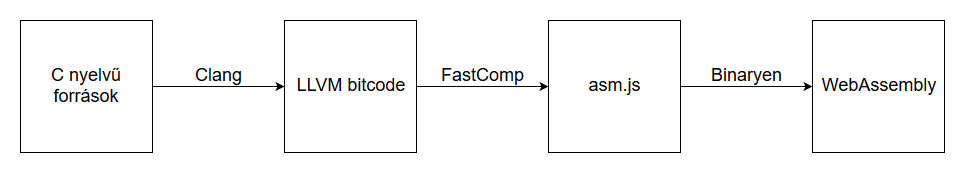
\includegraphics[width=\textwidth]{04-webassembly/emscripten-c-to-wasm.png}
    \caption{C $\rightarrow$ Wasm fordítás Emscriptennel.}
    \label{Figure::WebAssembly::EmscriptenCToWebAssembly}
\end{figure}

A folyamat első lépéseként a Clang fordító az LLVM belső reprezentációjára hozza az eredeti C nyelvű forrásokat. Ez egy könnyen optimalizálható formátum, melyből a FastComp asm.js kimenetet állít elő. Habár ez a köztes lépés nem lenne feltétlenül szükséges, azonban a köztes reprezentációból WebAssemblyt készítő LLVM \textit{backend} még instabilnak tekinthető, így egyelőre érdemesebb ezt az utat választani. A folyamat utolsó lépése a tényleges WebAssembly modul elkészítése, melyről a Binaryen gondoskodik. Természetesen a köztes lépések a felhasználó elől rejtve zajlanak.

Visszatérve a példához, a \texttt{library.c} fordításához szükséges parancsot a \dotref{Listing::WebAssembly::CompileWithEmscripten} kódrészlet tartalmazza. Az \texttt{EXPORTED\_FUNCTIONS} kapcsolóval külön meg kell adnunk a modul kliensei által is látható függvények listáját.

\begin{lstlisting}[language=bash, caption={A \texttt{library.c} fordítása Emscriptennel.}, captionpos=b, label=Listing::WebAssembly::CompileWithEmscripten, numbers=none]
emcc library.c -o library.js \ 
     -s EXPORTED_FUNCTIONS='["_factorial"]' \
     -s EXTRA_EXPORTED_RUNTIME_METHODS='["cwrap"]'
\end{lstlisting}

A futás eredményeként két fájl áll elő: a \texttt{library.wasm} és a \texttt{library.js}. Előbbi a C könyvtárból készült Wasm modul, míg utóbbi egy segédeszközöket tartalmazó JavaScript fájl, mely megkönnyíti a modul JavaScriptből történő felhasználását.

\subsection{Beágyazás HTML-be}

Az elkészült modul HTML kódba történő beágyazását a \dotref{Listing::WebAssembly::EmbeddingHTML} kódrészlet szemlélteti. Ezt egy HTML fájlként elmentve, majd megfelelő (azaz WebAssemblyt támogató) böngészőben megnyitva a „\textit{The factorial of 3 is 6.}” szöveget fogjuk látni.

\begin{lstlisting}[language=HTML, caption={A beágyazó HTML kód.}, captionpos=b, label=Listing::WebAssembly::EmbeddingHTML]
<!doctype html>
<html lang="en">
<head>
    <meta charset="UTF-8">
    <title>Factorial</title>
</head>
<body>
    <p id="result"></p>
    <script type="text/javascript">
        var Module = {
            onRuntimeInitialized() {
                const factorial = Module.cwrap('factorial', 'number', ['number'])

                document.getElementById('result').textContent =
                    `The factorial of 3 is ${factorial(3)}.`
            }
        }
    </script>
    <script async src="library.js"></script>
</body>
</html>
\end{lstlisting}

Ugyan a modul beágyazása a 19. sorban található \texttt{script} elemben történik, ez még csupán a WebAssembly kód feldolgozásáról, validálásáról és JIT vagy AOT fordításáról gondoskodik.

A \texttt{factorial} függvény tényleges futtatásának módját a 12-15. sorokban láthatjuk. Először a 12. sorban a \texttt{cwrap} függvény segítségével egy JavaScript függvényt készítünk az exportált \texttt{factorial} függvényből. A \texttt{cwrap} az exportált függvény neve mellett annak visszatérési típusát, valamint paramétereinek típusát várja. Ezt követően a visszaadott függvény már a szokásos JavaScript függvényekkel azonos módon hívható, amit a 15. sorban láthatunk.

Érdemes még a beágyazó kódban található \texttt{Module} objektumot is megemlíteni (10. sor). Alapesetben az Emscripten által kibocsátott segédkönyvtár egy \texttt{Module} nevű objektumot exportál. Ugyanakkor, ha a beágyazó kód már tartalmaz egy ilyen nevű változót, akkor a segédkönyvtár ezt fogja felhasználni. Az ezen az objektumon definiált \texttt{onRuntimeInitialized} függvény akkor kerül meghívásra, amikor a WebAssembly modul elérhetővé vált, azaz a futtató környezet felkészült a kódvégrehajtásra.

    \chapter{CryptID}

Az előző fejezetek előbb a kriptográfiai, majd a technológiai alapokat vezették be. Ebben a fejezetben a dolgozat eredményét jelentő programkönyvtár – a CryptID – kerül részletesen ismertetésre.

A fejezet felépítése a következő: Először magas szinten vázoljuk, hogy mi is pontosan a CryptID, miben jelent újdonságot, milyen megfontolások állnak mögötte. Ezt követi a könyvtár struktúrájának alapos bemutatása, rétegről rétegre haladva. Az utolsó előtti szekció egyfajta útmutatóként szolgál a CryptID felhasználásához, integrálásához. Végül a fejezetet a könyvtár teljesítményének elemzése zárja.


\section{Mi a CryptID?}

A CryptID egy nyílt forrású IBE megoldás, mely az RFC 5091-ben meghatározott Boneh-Franklin sémát veszi alapul. Újszerűsége két irányból is megközelíthető, egyrészt az implementációt, másrészt az IBE sémát tekintve. 

A megvalósításban rejlő újdonság, hogy a CryptID WebAssembly alapokon működik, aminek köszönhetően nemcsak a szerveroldalon, hanem a kliensoldalon, vagy akár a webtől teljesen elszakadva nyújt platformfüggetlen és hatékony titkosítási megoldást.

Az IBE sémához hozzátett újítás a publikus kulcsban keresendő. A CryptID strukturált publikus kulcsokra épül, melyekben az egyedi azonosítón felül tetszőleges metaadat elhelyezhető.

A következőkben az előbb felsorolt sajátosságokat fejtjük ki részletesen, mindenütt kitérve a háttérben álló motivációkra is.

\subsection{Platformfüggetlen működés}

A CryptID formájában egy olyan könyvtárat szerettünk volna létrehozni, mely hatékony kliensoldali titkosítást tesz lehetővé. Mindezt olyan formában szerettük volna megvalósítani, hogy ugyanaz a megoldás alkalmazható legyen asztali gépeken, tableteken és mobiltelefonokon egyaránt. Ezt az erőfeszítést az a motiváció hajtotta, hogy nem tudunk olyan nyílt forrású IBE könyvtárról, mely módosítás nélkül (\textit{out-of-the-box}) használható lenne ezen platformok mindegyikén.

Adott volt tehát a célkitűzés: egy böngészőben futtatható, hatékony programkönyvtár létrehozása. Korábban a JavaScript volt az egyetlen olyan technológia, mely ilyen mértékű platformfüggetlenséget kínált. Azonban az egyes böngészőkben található JavaScript motorok jelentősen eltérő optimalizációkat alkalmazhatnak, így ami az egyik böngészőben gyorsan fut, az elképzelhető, hogy egy másikban jóval gyengébb teljesítményt nyújt. Erre a problémára ugyan megoldást kínál az asm.js, mely egyszerűségénél fogva könnyebben és egyértelműbben optimalizálható, azonban ez korántsem tekinthető szilárd és jól támogatott szabványnak.

Rátaláltunk azonban az előző fejezetben ismertetett WebAssembly szabványra, mely pontosan azt nyújtotta, amire szükségünk volt: hordozható binárist és gyors végrehajtást. A WebAssemblynek köszönhetően kihasználhattuk azt is, hogy C-ben számos régóta fejlesztett és alaposan tesztelt matematikai, illetve kriptográfiai programkönyvtár áll rendelkezésre. Ilyen a GMP \cite{GMP} és az OpenSSL \cite{OpenSSL} is, melyek a CryptID alapját képzik.

\subsection{Strukturált publikus kulcs}

Az IBE lényege, hogy a publikus kulcs egy adott domainen belül valamilyen entitást egyértelműen azonosít. Legegyszerűbb példa erre egy email cím, vagy adott rendszeren belüli felhasználónév. Boneh és Franklin azonban a róluk elnevezett sémát leíró cikkükben \citeyear{Boneh::IdentityBasedEncryptionFromTheWeilPairing} említenek olyan alkalmazásokat is, melyek a publikus kulcsot további metaadatokkal egészítik ki. Ilyen metaadat lehet például az aktuális év, mely egyfajta érvényességet rendel a publikus kulcshoz és így áttételesen a hozzátartozó privát kulcshoz is. Az említett cikkben ez a metaadat egyszerűen az azonosítóhoz konkatenálva jelenik meg a publikus kulcsban: „\texttt{bob@company.com $\parallel$ current-year}”.

A metaadatok beágyazásának ötletét nagyszerűnek találtuk, azonban úgy éreztük, hogy a konkatenáció szükségtelen kötöttséget erőltet a publikus kulcsra: az egyes mezőknek mindig azonos sorrendben kell szerepelniük. Természetesen ezen közvetlenül nem változtathatunk, hiszen a titkosítás, majd a visszafejtés csak akkor működik az elvártnak megfelelően, ha a publikus kulcs mindig bitpontosan azonos.

E megszorítást csak az absztrakció szintjének megemelésével kerülhettük meg. A \mbox{CryptID} ennek folytán JavaScript objektumokat használ publikus kulcsként. Az objektumok publikus kulcsra történő leképezése a könyvtár implementációs részletei közé tartozik, ezzel a CryptID-et integráló fejlesztőnek nem kell foglalkoznia. Ily módon a CryptID megszünteti a sorrendi kötöttség okozta terhet, mi több, a fejlesztőknek azzal sem kell törődniük, hogy a publikus kulcsot reprezentáló objektumból hogyan lesz bitsorozat – a konverzió a kulisszák mögött történik.

\subsection{Nyílt forrású, RFC-alapú implementáció}

Egy adott kriptorendszerhez megbízható implementációt készíteni rendkívül nehéz feladat. Hiába áll ugyanis rendelkezésünkre egy matematikailag bizonyítottan biztonságos kriptorendszer, annak megvalósítása során könnyen véthetünk olyan hibákat, melyek sebezhetőségeket nyitnak. Ezek a sebezhetőségek fakadhatnak például programozási hanyagságból (például a bemenet nem megfelelő ellenőrzése), vagy matematikai figyelmetlenségből, tudatlanságból (támadható elliptikus görbe használata).

Számos gyakori hiba megelőzhető azonban, ha valamilyen nyílt szabvány vagy ajánlás alapján készítjük el az implementációnkat. A CryptID esetében is így tettünk: az RFC 5091-et használtuk fel, mely a Boneh-Franklin és a Boneh-Boyen IBE rendszerek lehetséges implementációját írja le egy bizonyos szuperszinguláris elliptikus görbe felett \cite{RFC5091}. Ezek közül a CryptID a Boneh-Franklin rendszerre épül.

Az említett RFC részletes pszeudokódot biztosít az IBE-t felépítő főbb algoritmusokhoz (\textit{Setup, Extract, Encrypt, Decrypt}, és alacsonyabb szintű társaik), ajánlásokat ad öt biztonsági szintre vonatkozóan (vö. \dotref{table::RFC::SecurityParam} táblázat), lehetővé téve ezzel a rendszer parametrizálását, valamint tesztadatokat tartalmaz, melyek elősegítik az implementációk tesztelését. Ezek a tesztadatok hatalmas segítséget jelentettek a fejlesztés során, hiszen a teljes rendszer lekódolása előtt meg tudtunk bizonyosodni az azt felépítő kisebb rutinok helyes működéséről is.

A CryptID nemcsak az ajánlásnak megfelelő, hanem egyúttal nyílt forrású is. Természetesen a nyílt forrású szoftverek nem lesznek automatikusan biztonságosabbak, mint zárt forrású társaik, azonban a transzparenciának köszönhetően a kód könnyebben és többek által átvizsgálható és ellenőrizhető, így összességében a nyílt forrás hozzájárulhat a megbízhatóbb implementáció létrejöttéhez \cite{Wheeler::SecureProgrammingForLinuxAndUnixHOWTO}.

\pagebreak


\section{A CryptID felépítése}

Magas szintről szemlélve, a CryptID három komponensből áll:

\begin{outdentlist}
    \item[]\textbf{CryptID.ref.}
    Java nyelven írt referencia-implementáció. Az egyetemi tanulmányaink során leggyakrabban a Java nyelvvel volt alkalmunk dolgozni, ennek folytán Javaban rendelkezünk a legmagabiztosabb tudással. Ezt kihasználva, először elkészítettük az IBE Java nyelvű megvalósítását, melyet aztán felhasználhattunk a WebAssembly implementáció helyességének ellenőrzéséhez.

    \item[]\textbf{CryptID.wasm.}
    Az IBE-t alkotó rutinokat tartalmazó WebAssembly modul. A forrásnyelv C, ezt fordítjuk át Emscripten segítségével WebAssemblyre (ld. \dotref{Subsection::WebAssembly::Forditas}).

    \item[]\textbf{CryptID.js.}
    A WebAssembly modult becsomagoló JavaScript könyvtár, mely egy könnyen használható interfészen keresztül teszi elérhetővé az IBE rutinokat.
\end{outdentlist}

E három komponens valójában két különálló, bár szemantikát tekintve azonos IBE-megoldást alkot. Az egyiket a CryptID.ref önmagában, míg a másikat a CryptID.wasm és arra építve a CryptID.js. A továbbiakban a CryptID.ref ismertetését elhagyjuk, és a CryptID néven a CryptID.wasm és a CryptID.js komponensek együtteséből formált könyvtárra fogunk hivatkozni. E könyvtár struktúráját az \dotref{Figure::CryptID::Stack} ábra szemlélteti.

\begin{figure}[h]
    \centering
    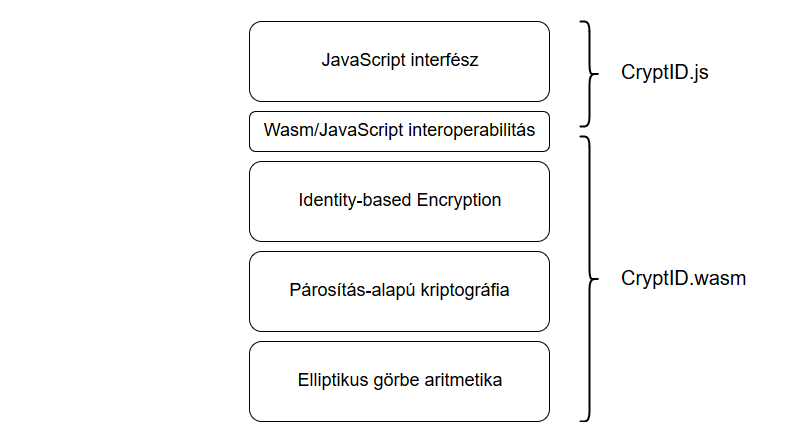
\includegraphics[height=225px]{05-cryptid/stack-smaller-gaps-box-centered.png}
    \caption{A CryptID felépítése.}
    \label{Figure::CryptID::Stack}
\end{figure}

A következőkben lentről felfelé haladva részletesen bemutatjuk az egyes rétegeket.

\subsection{Elliptikus görbe aritmetika}

Az IBE egy elliptikus görbe kriptográfián alapuló titkosítási rendszer, ezért az elliptikus görbe aritmetika képzi a CryptID magját is. A \ref{Chapter::ECC}. fejezetben összefoglaltuk az elliptikus görbék legfontosabb matematikai tulajdonságait, dolgozatunk ezen részében pedig az implementációhoz szükséges ismereteket tárgyaljuk.

Az elliptikus görbék matematikai háttere hosszú múltra tekint vissza, és számos elliptikus görbe aritmetikát megvalósító könyvtár áll rendelkezésre. Természetesen merül fel a kérdés, hogy ezek ellenére miért készítettünk saját implementációt?

Úgy találtuk, hogy az általunk vizsgált könyvtárak mindegyike rendelkezett olyan negatív tulajdonsággal (jelentős méret, átláthatatlan implementáció, hiányos dokumentáció), ami miatt úgy döntöttünk, hogy egy saját, pehelysúlyú réteget hozunk létre, ami megfelel minden elvárásunknak.

\subsubsection{Elliptikus görbe aritmetika tulajdonságai}

Az elliptikus görbe aritmetikát megvalósító rétegnek a legfontosabb tulajdonsága, hogy az RFC 5091-ben ajánlott \textit{Type-1} elliptikus görbékre van optimalizálva. A \textit{Type-1} osztály olyan görbéket takar, melyek alakja $E(\mathbb{F}_p) : y^2 = x^3 + 1$, ahol  $p \equiv 11 (\bmod \; 12)$ tetszőleges prím. Ezek a görbék a szuperszinguláris görbék egy részcsoportját képezik.

Az $\mathbb{F}_p$-beli elemek ábrázolására a GMP aritmetikai könyvtár véges test támogatását használtuk fel, ami egy rendkívül kiforrott és jól tesztelt megoldást nyújt.

A réteg képes $\mathbb{F}_{p^2}$-beli elemek ábrázolására is, amelyek lényegében $\mathbb{F}_p$-beli elemek rendezett párjai. Egy ilyen rendezett párt jelölünk $(a_0, a_1)$-el, amit értelmezhetünk az $a_0 + a_1 \cdot i$ komplex számnak, ahol $i^2 = -1$. 

Ezzel az értelmezéssel egyszerűen a komplex aritmetikát alapul véve végezhetünk műveleteket $\mathbb{F}_{p^2}$ felett, annyi különbséggel, hogy minden esetben moduloját kell venni az eredményeknek, hogy a műveletek zártak maradjanak. Az ilyen műveletek kivitelezését a GMP alapú $\mathbb{F}_p$ test feletti aritmetikára építve végeztük el. 

Implementálásra került $\mathbb{F}_{p^2}$ feletti elemek egymással és skalárral vett összeadása, additív inverz képzése, elemek egymással és skalárral való szorzása, hatványozása egész számmal és multiplikatív inverz képzése.

Az említett $\mathbb{F}_{p^2}$ aritmetika implementálására azért volt szükség, mert a kriptográfiában az egyszerű Tate párosítás gyakran nem alkalmazható. Ugyanakkor, ha módosítjuk annyiban, hogy az egyik bemenete egy torzítási leképezése az elliptikus görbe egy pontjának, akkor biztosan két egymástól lineárisan független ponttal dolgozhatunk, kizárva az elfajultságot.

\subsubsection{Elliptikus görbe pontjainak ábrázolása}

A réteg két lehetőséget nyújt a görbe pontjainak ábrázolására. Egyik az affin térben való ábrázolás, a másik lehetőség pedig a projektív tér használata. Egy alap IBE implementációhoz elegendő lenne az affin pontábrázolás is, azonban a projektív koordináták használata egyszerű optimalizációs lehetőségeket nyújt.

Fontos megjegyezni, hogy több módja is van a projektív pontábrázolásnak, melyek közül mi az RFC 5091 ajánlását követve a Jacobi projektív módszert implementáltuk. Amíg az affin ábrázolás esetében a pontunkat egy $(x, y)$ számpáros alkotja, a Jacobi projektív módszer egy $(x, y, z)$ számhármast használ.

Miben is rejlik az utóbbi módszer hatékonysága? Nos, ha $M, S$ és $I$ rendre a szorzás, négyzetre emelés és invertálás műveleteit jelölik, akkor az \dotref{table::OperationCost} táblázatban látható, hogy az egyes módszerek és görbe műveletek esetén melyik test-műveletet hányszor kell végrehajtani.

A lényegi különbséget az invertálás elhagyása jelenti a görbe műveletek esetén, mert a szorzás és invertálás számításigényének aránya általánosan $80 : 1$ \cite{Nyakacska::ECC-PBC}, míg a szorzás és négyzetre emelés esetén $10 : 8$ \cite{BernsteinLange::ECC}.

\begin{table}[H]
    \centering
    \begin{tabular}{|l|l|l|}
    \hline
    \textbf{Pontábrázolás típusa} & \textbf{Összeadás} & \textbf{Duplázás} \\ \hline
    affin                         & $I + 2M + 2S$      & $I + 2M + 1S$     \\ \hline
    Jacobi projektív              & $12M + 4S$         & $4M + 6S$         \\ \hline
    \end{tabular}
    \caption{Elliptikus görbén végzett műveletek költsége \protect\cite{Martin::IntroductionToIdentityBasedEncryption}.}
    \label{table::OperationCost}
\end{table}

A tárgyalt ábrázolási módok mindegyikével a következő elliptikus görbe műveletek végezhetők:

\begin{outdentlist}
    \item[]\textbf{Pont duplázás.}
    Egyszerű pont duplázást megvalósító algoritmus, melyet a Martin könyvében leírtak alapján implementáltunk.
    
    \item[]\textbf{Pont összeadás.}
    Az implementált algoritmus forrása megegyezik a duplázás esetében használttal.

    \item[]\textbf{Pont szorzása skalárral.} 
    A \textit{Double-and-Add} algoritmust megvalósító skaláris szorzás került implementálásra a rétegben, ami megfelelőnek mondható, de még optimalizálható sebességet nyújt.
    
    \item[]\textbf{Pontábrázolások közötti konverzió.}
    A réteg részét képezi a két említett pontábrázolás közötti konverzió, ami affinból Jacobi projektívbe való átalakítás esetén $(x, y) \rightarrow (x, y, 1)$, fordított irányban pedig $(x, y, z) \rightarrow (x/z^2, y/z^3)$ módosítást végez.
\end{outdentlist}

\subsection{Párosítás-alapú kriptográfia}

A BF-IBE-nek és így a CryptID-nek is kihagyhatatlan része a párosítás műveletének megvalósítása. Az RFC 5091 ajánlását követve a réteg a Tate párosítást tartalmazza.

Az implementált Tate párosítás két $E(\mathbb{F}_p)$-beli pontot képez le egy $\mathbb{F}_{p^2}$-beli elemre. Az implementációt az RFC 5091 \citeyear{RFC5091}, Martin könyve \citeyear{Martin::IntroductionToIdentityBasedEncryption} és Lynn doktori disszertációja \citeyear{Lynn::PBC} alapján készítettük el.

\subsection{Identity-based Encryption}

A CryptID fő funkcionalitását megvalósító réteg. Tartalmazza a BF-IBE négy fő függvényét (\textit{Setup}, \textit{Extract}, \textit{Encrypt}, \textit{Decrypt}), amelyeket az Identity-based Encryption című fejezetben ismertettünk.

Az implementáció során az RFC 5091 ajánlásait követtük, amelyek nem csupán az említett függvénynégyesre vonatkoznak, hanem az azok működtetéséhez szükséges algoritmusokra is. 

Ilyenek az Identity-based Encryption című fejezet pszeudokódjaiban megjelent hash függvények:

\begin{outdentlist}
    \item[]\textbf{H1 - \textit{hashToPoint}} $\{0, 1\}^* \rightarrow G_1$
    
    \item[]\textbf{H2 - \textit{canonical}} $G_\mathbb{T} \rightarrow \{0, 1\}^n$
    
    \item[]\textbf{H3 - \textit{hashToRange}} $\{0, 1\}^n \times \{0, 1\}^n \rightarrow \mathbb{Z}_q$
    
    \item[]\textbf{H4 - \textit{hashBytes}} $\{0, 1\}^n \rightarrow \{0, 1\}^n$
\end{outdentlist}

A felsorolt hash függvények alapját a \textit{canonical} kivételével a Secure Hash Algorithms (SHA) hash függvény alkotja, amelyet számunkra az OpenSSL könyvtár biztosított. Az előbbi könyvtárat nem csupán az SHA implementációja miatt használjuk, hanem a kriptográfiailag biztonságos és jól tesztelt random szám generátora is nagy segítséget nyújtott számunkra.

\subsection{Wasm/JavaScript interoperabilitás}

A megelőző három réteg együttesen egy C nyelvű IBE implementációt alkot, mely akár WebAssemblyre történő fordítás nélkül is felhasználható, például natív alkalmazások készítéséhez. Természetesen a CryptID-ben nem mint natív könyvtár, hanem mint WebAssembly modul kerülnek elhelyezésre ezek a rétegek, egy JavaScript interfész mögé rejtve.

Felmerülhet a kérdés, hogy miért szükséges egy ilyen absztrakció, ha egyszer a WebAssemblyt beágyazó környezetek közvetlenül is lehetővé teszik a modulban definiált függvények meghívását? A válasz erre kettős: Egyfelől nincsen rá szükség, a CryptID.wasm önmagában is felhasználható. Másfelől viszont, a CryptID-et elsősorban olyan beágyazó környezetekben történő felhasználásra szánjuk, melyek JavaScripten keresztül teszik lehetővé a WebAssembly modulok meghívását. Ilyen környezet például a böngésző vagy a Node.js. Ezekben a környezetekben nagy segítséget jelent, hogy a CryptID ugyanúgy hívható, mint bármely más, JavaScriptben írt könyvtár, a WebAssembly pedig csupán implementációs részlet marad. 

E megközelítés támogatásához, még a JavaScript interfész alatt megtalálható egy úgynevezett interoperabilitási (röviden: interop) réteg, melynek egyik fele C-ben, másik fele pedig JavaScriptben készült. Az említett réteg a következő feladatokat látja el:

\begin{outdentlist}
    \item[]\textbf{C függvények becsomagolása.}
    Ahhoz, hogy a C-ben írt függvények JavaScriptből hívhatók legyenek, be kell csomagolni őket az Emscripten által biztosított \texttt{Module} objektum \texttt{cwrap} metódusa segítségével. Az interop réteg gondoskodik a WebAssembly-oldalon exportált összes függvény helyes becsomagolásáról.

    \item[]\textbf{Adattípusok közötti konverzió.}
    A C-ben készült IBE függvények két olyan adattípust is felhasználnak, melyek konverziót igényelnek:

    \begin{itemize}
        \item
        Míg a JavaScript-oldal a nagy egészeket karakterláncok formájában kezeli (adott számrendszerben reprezentálva az értéket), addig C-ben a GMP könyvtár \texttt{mpz\_t} típusa használatos. E két típus között kétirányú konverzióra van szükség (hiszen a nagy egészek kimenetet és bemenetet is jelenthetnek), melyet a GMP \texttt{mpz\_get\_str}\footnote{\url{https://gmplib.org/manual/Converting-Integers.html#Converting-Integers}} és \texttt{mpz\_init\_set\_str}\footnote{\url{https://gmplib.org/manual/Simultaneous-Integer-Init-_0026-Assign.html}} függvényeinek felhasználásával valósítottunk meg.

        \item
        A titkosítást implementáló C függvény a \texttt{CipherTextTuple} típus egy példányát állítja elő, mely nyers bájtsorozatokat is tartalmaz. Habár JavaScriptben az \texttt{ArrayBuffer}\footnote{\url{https://developer.mozilla.org/en-US/docs/Web/JavaScript/Reference/Global_Objects/ArrayBuffer}} lehetővé teszi a bináris adatok hatékony kezelését, azonban a továbbítás vagy mentés legtöbbször nem nyers formában történik. Ennek elősegítésére az interop réteg Base64 kódolásúra\footnote{\url{https://tools.ietf.org/html/rfc4648#section-4}} alakítja a \texttt{CipherTextTuple} bináris tartalmát.
    \end{itemize}

    \item[]\textbf{Kétirányú adatáramlás biztosítása.}
    A WebAssembly modulok egy vagy több elkülönített, lineáris memóriát használhatnak \cite{WebAssemblySpecification}. A böngészőben történő beágyazás esetében ezek a memóriaterületek a JavaScript kód által használt memóriától izoláltan kerülnek lefoglalásra. Mivel közvetlenül nem lehetséges az összetett típusok (például a különböző \texttt{struct} típusok) paraméterként vagy visszatérési értékként való használata, ezért ezen típusok példányait csak a WebAssembly és a JavaScript által birtokolt memóriaterületek közötti másolással lehet kicserélni. Ennek megfelelő lebonyolítása magában foglalja a lineáris memória JavaScript oldalról történő írását és olvasását, valamint a C oldalon történő helyes memóriafoglalást és -felszabadítást.
\end{outdentlist}

\subsection{JavaScript interfész}

A JavaScript interfész jelenti a CryptID külvilág számára nyilvános függvényeit és adattípusait. Míg a megelőző rétegek implementációs részletnek tekinthetők, addig erre az interfészre a kliensek közvetlenül is támaszkodhatnak. 

\subsubsection{Felelősségi körök}

Azon felül, hogy az interfész kapcsolatot jelent a könyvtár alsóbb rétegei és az integráló kliens között, további felelősségi köröket is ellát:

\begin{outdentlist}
    \item[]\textbf{A bemenet ellenőrzése.}
    Mivel ez a réteg választja el a könyvtár megvalósítását a külvilágtól, ez az egyetlen olyan pont, ahol hibás adatok léphetnek be a rendszerbe. Ilyen hibás bemenetre számtalan példa adható, elég ha a \texttt{null} értékekre, a nem megfelelő alakú objektumokra vagy a hibásan kódolt adatokra gondolunk. Az ilyen rendellenes inputok kiszűrése ebben a rétegben történik, mielőtt még bármilyen számítás alapját képezhetnék.

    \item[]\textbf{Kulcskonverzió.}
    A CryptID jelentette újdonságok közül az egyik a strukturált, metaadatokat tartalmazó publikus kulcs, melyet a könyvtár egy JavaScript objektum formájában vár. Fontos követelmény azonban, hogy a tartalmilag azonos JavaScript objektumokból mindig azonos bitsorozatot kell előállítani.
    
    Naiv megoldása lehetne ennek a problémának a következő: először a \texttt{JSON.stringify} függvény segítségével karakterláncot képzünk az objektumból, majd ezt egyszerű bitsorozatként interpretáljuk (azaz \texttt{char[]} típusként C-ben). E megközelítés azonban tartalmilag azonos objektumok esetén eltérő karakterláncokat eredményezhet, abból kifolyólag, hogy a \texttt{JSON.stringify} az objektumok kulcsait azok hozzáadásának sorrendjében konvertálja \cite{ECMAScript2015Specification}.
    
    Ezt megkerülendő, a \texttt{JSON.stringify} meghívása előtt a CryptID a publikus kulcsként szolgáló objektumból létrehoz egy vele tartalmilag azonos objektumot, melyhez azonban a kulcsok betűrendben kerülnek hozzáadásra. E konverziónak köszönhetően a JavaScript interfész alatti rétegek már egy bitsorozatot kapnak publikus kulcsként, a strukturáltsággal tehát egyáltalán nem kell foglalkozniuk.
\end{outdentlist}

\subsubsection{Exportált típusok}

A JavaScript interfész által exportált összes típus WebIDL\footnote{\url{https://www.w3.org/TR/WebIDL-1/}} definíciója megtalálható a CryptID – WebIDL definíciók függelékben,
% ref majd hozzá
a tényleges funkcionalitást biztosító két interfész azonban a könnyebb áttekinthetőség kedvéért az \dotref{Listing::CryptID::WebIDLInterfaces} kódrészletben is megtalálható.

\lstinputlisting[language=WebIDL, caption={A funkcionalitást biztosító interfészek.}, captionpos=b, label=Listing::CryptID::WebIDLInterfaces, firstline=1, lastline=21]{./code/cryptid.webidl}

Az integráló kód számára a könyvtár a \texttt{CryptIDFactory} interfész példányaként jelenik meg. Ezen interfész egyetlen függvénye az objektumgyárként (\textit{factory}) funkcionáló \texttt{getInstance}, mely a \texttt{CryptID} példányok aszinkron létrehozására képes. A \textit{factory} metódus által biztosított indirekció lehetővé teszi, hogy a visszaadott interfész mögé más és más implementáció kerüljön; például WebAssemblyt nem támogató böngésző esetén egy asm.js megvalósítás. Az aszinkronitás pedig annak enged utat, hogy a hívó kód futása a példány előállítása közben is folytatódhasson. E módon lehetséges például a WebAssembly kód lusta (\textit{lazy}) betöltése: a Wasm bináris nem kerül letöltésre a weboldal többi részével együtt, hanem csak a \texttt{getInstance} függvény meghívásakor indul el a háttérben a letöltés, feldolgozás és validálás.

Az IBE-hez kapcsolódó rutinokat a \texttt{CryptID} interfészen találjuk. E függvények visszatérési értéke minden esetben tartalmaz egy \texttt{success} nevű mezőt, mely a kívánt művelet sikerességét jelzi. Ha például a \texttt{decrypt} metódust nem a megfelelő privát kulccsal hívjuk, akkor a visszaadott objektum \texttt{success} mezője \texttt{false} értéket fog felvenni. Azért választottuk ezt a megoldást a kivételekkel szemben (és valójában mellett), mert a kivételeket valóban a kivételes esetek számára tartjuk fent \cite{Bloch::EffectiveJava}, mint például a hibás bemeneti formátumok, a megsértett invariánsok vagy a váratlan számítási hibák. Úgy gondoljuk, hogy e módon egy könnyebben integrálható, kényelmesebb felületet tudunk biztosítani a kliensek számára.

Érdemes még megemlíteni a \texttt{dispose} függvényt, mely a \texttt{CryptID} interfész által lefoglalt erőforrások elengedésére, felszabadítására szolgál. Ilyen erőforrás lehet például a WebAssembly implementáció esetén a modul által használt memóriaterület. Ha már nincs szükségünk IBE rutinokra, akkor érdemes a \texttt{dispose} segítségével a lehető leghamarabb felszabadítani a nem használt erőforrásokat. A \texttt{dispose} hívását követően bármelyik, az adott példány által biztosított függvény meghívása (beleértve magát a \texttt{dispose}-t is) hibának számít, és kivételt eredményez. 

\section{Alkalmazásfejlesztés CryptID-del}
\label{Section::CryptID::ApplicationDevelopment}

A következőkben a könyvtár alapszintű felhasználását mutatjuk be egy JavaScript program formájában. Ennek célja, hogy illusztrálja a CryptID integrálásának egyszerű voltát. A könnyebb olvashatóság érdekében a programot kisebb kódrészletekre bontva ismertetjük, a CryptID – Példaprogram függelékben
% megfelelő hivatkozás
azonban egyben is megtalálható a teljes forráskód.

Előbb a biztosított funkcionalitás rövid leírását adjuk, amit aztán a forráskód és az ahhoz fűzött magyarázatok követnek. 

\subsection{Funkcionalitás}

A példaprogram által megvalósított funkcionalitás a következő: Először új nyilvános paramétereket és mesterkulcsot generál. Ezt követően egy előre rögzített üzenetet titkosít egy email címet tartalmazó nyilvános kulccsal. A titkosítás után előállítja a nyilvános kulcshoz tartozó privát kulcsot, végül pedig ennek használatával visszaállítja az eredeti üzenetet a titkos szövegből.

\subsection{Implementáció}

\textit{Szeretnénk felhívni a figyelmet arra, hogy az olvashatóság megőrzése érdekében a következő kódrészletek nem tartalmaznak hibakezelést. Ezen felül kiemelnénk, hogy a sorok számozása folytonos, azaz a mindenkori sorszám a teljes forrásban elfoglalt pozíciót tükrözi.}

\lstinputlisting[language=JavaScript, firstline=1, lastline=2, escapechar=^]{./code/application-development-with-cryptid.js}

Az első teendőt a felhasznált könyvtárak importálása jelenti. A \texttt{perf\_hooks} a futási idő mérésére szolgáló rutinokat biztosít, míg a a \texttt{cryptid} a korábban említett \texttt{CryptIDFactory} interfész egy példányát exportálja.

\lstinputlisting[language=JavaScript, firstline=4, lastline=7, escapechar=^, firstnumber=4, showstringspaces=false]{./code/application-development-with-cryptid.js}

Mind az üzenet, mind a publikus kulcs rögzített értékkel bír. A publikus kulcs egy JavaScript objektum, mely metaadatokat ezúttal nem, csupán egy azonosításra használható email címet tartalmaz. Ennek valódi szerepe ugyanakkor jelenleg nincsen, hiszen az azonosító ellenőrzése nem része a példaprogramnak.

\lstinputlisting[language=JavaScript, firstline=9, lastline=10, escapechar=^, firstnumber=9, showstringspaces=false]{./code/application-development-with-cryptid.js}

Az IBE függvények a \texttt{CryptID} interfészen találhatók, melynek példányait a \texttt{CryptIDFactory} interfész által definiált \texttt{getInstance} metódus képes előállítani. Ennek végrehajtása aszinkron, ezért a JavaScript \texttt{async-await} szintaxisát használjuk a visszatérési érték kinyeréséhez.

\lstinputlisting[language=JavaScript, firstline=12, lastline=15, escapechar=^, firstnumber=12, showstringspaces=false]{./code/application-development-with-cryptid.js}

Amennyiben még nem rendelkezünk publikus paraméterekkel és mesterkulccsal, akkor le kell generálnunk őket. Erre szolgál a \texttt{setup} függvény, melynek egyetlen paramétere a titkosítás erősségét határozza meg. Ezúttal a \texttt{lowest} beállítást választjuk, mely gyenge titkosítást, ugyanakkor rendkívül gyors futást garantál.

Az alkalmazás az IBE rutinok végrehajtási idejét is leméri a rutinok futása előtt és után rögzített időbélyegek segítségével. Az előbbi időbélyeget a \texttt{setup} függvényt megelőzően hozzuk létre, majd eltároljuk a \texttt{start} változóban.

\lstinputlisting[language=JavaScript, firstline=17, lastline=17, escapechar=^, firstnumber=17, showstringspaces=false]{./code/application-development-with-cryptid.js}

Publikus paraméterek birtokában már lehetséges az üzenet letitkosítása. Ehhez még szükséges egy nyilvános kulcs is, melyet jelen esetben a \texttt{PUBLIC\_KEY} változó tárol. Sikeres végrehajtás esetén a visszaadott objektum \texttt{ciphertext} mezője tartalmazza a titkos szöveget.

\lstinputlisting[language=JavaScript, firstline=19, lastline=19, escapechar=^, firstnumber=19, showstringspaces=false]{./code/application-development-with-cryptid.js}

A titkos szöveg visszafejtése csak egy privát kulcs birtokában lehetséges, melyet az \texttt{extract} függvény hívásával generálhatunk. Fontos kihangsúlyozni, hogy a nyilvános kulcsban szereplő adatok ellenőrzését ez a függvény nem végzi el, arról a kliensnek kell gondoskodnia.

\lstinputlisting[language=JavaScript, firstline=21, lastline=22, escapechar=^, firstnumber=21, showstringspaces=false]{./code/application-development-with-cryptid.js}

Az eredeti üzenet visszaállításának utolsó lépését a titkos szöveg visszafejtése jelenti. Ez csak akkor lehet sikeres, ha az üzenet titkosításához használt nyilvános kulcs privát párját használjuk. Mivel a példaprogramban ez biztosan teljesül, ezért a \texttt{decrypt} hívása az eredeti üzenettel fog visszatérni, melyet a \texttt{plaintext} változóban tárolunk.

A végrehajtási idő mérésének végét jelentő időbélyeg rögzítése is ekkor történik meg. A \texttt{runningTime} változó a futás alatt eltelt ezredmásodperceket fogja tartalmazni.

\lstinputlisting[language=JavaScript, firstline=24, lastline=28, escapechar=^, firstnumber=24, showstringspaces=false]{./code/application-development-with-cryptid.js}

A forráskód utolsó soraiban a lefoglalt erőforrások felszabadítását, valamint a visszafejtett üzenet és a futási idő kiíratását találjuk. Habár a \texttt{dispose} meghívása jelen esetben nem feltétlenül szükséges (hiszen az alkalmazás végrehajtása után a lefoglalt erőforrások automatikusan felszabadulnak), azonban böngészőben, vagy hosszabb futásra tervezett szerveroldali alkalmazásban kritikus lehet az erőforrásokkal való megfelelő gazdálkodás.

\section{Teljesítmény}
\label{Section::Performance}

A fejezet megelőző részeiben előbb megismerkedhettünk a könyvtár struktúrájával és implementációs részleteivel, majd a gyakorlathoz közelítve láthattuk az alapszintű használatát is. Mielőtt azonban bemutatnánk a CryptID segítségével építhető nagyobb léptékű alkalmazásokat, szeretnénk a könyvtár teljesítményét is vázolni.

A nemfunkcionális követelmények közül a teljesítmény, azon belül is a végrehajtási idő kritikus szereppel bír. Hiába rendelkezik ugyanis egy megoldás magas biztonsági garanciákkal, ha futási ideje olyan rossz, hogy a gyakorlatban használhatatlan. 

A következőkben különböző mérések útján a CryptID legfontosabb komponenseinek teljesítményét elemezzük, minden esetben kitérve az optimalizációs lehetőségekre is. A mérésekhez használt környezetek pontos jellemzői megtalálhatók a CryptID – Teljesítmény függelékben, csakúgy mint a használt metodológia, valamint a pontos mért értékek.

\subsection{Pont skaláris szorzása}

Az IBE-hez szükséges elliptikus görbe aritmetika központi eleme a skaláris szorzás. Ez a művelet számos könyvtárban megtalálható, melyek közül a korábban is említett MIRACL-t és a PARI-t választottuk ki a CryptID-del történő összehasonlításhoz. Összesen tehát négy implementációt hasonlítottunk össze: a natívan futó, C-ben írt MIRACL, PARI és CryptID megoldásokat, valamint a CryptID WebAssembly változatát.

Mivel mind a MIRACL, mind a PARI régóta fejlesztett, hatékony könyvtárnak tekinthető, ezért azt vártuk, hogy ezek biztosan gyorsabbak lesznek még a CryptID C változatánál is. Úgy gondoltuk, hogy az utolsó helyen a WebAssembly verzió fog állni.

\begin{figure}[h]
    \centering
    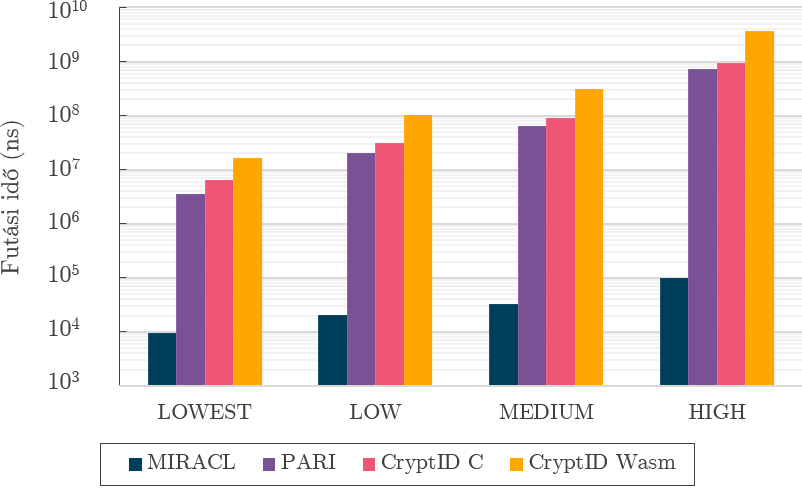
\includegraphics[height=225px]{05-cryptid/elliptic-multiplication-chart.png}
    \caption{Az elliptikus skaláris szorzás futási ideje.}
    \label{Figure::CryptID::EllipticMultiplicationChart}
\end{figure}

Az \dotref{Figure::CryptID::EllipticMultiplicationChart} ábrán logaritmikus skálára vetítve láthatjuk az egyes megoldások futási idejét különböző méretű bemenetekre. Az adatokból leolvasható, hogy az elvárásaink javarészt beigazolódtak: a MIRACL minden bemenet esetén nagyságrendekkel gyorsabban fut, mint a többi megoldás, és valóban a WebAssembly végrehajtása tart a legtovább. A MIRACL kitűnő teljesítményét többek között az implementált \textit{wNAF} algoritmus hatékonyságának köszönheti\footnote{\url{http://bit.ly/miracl-ecurve-mult}} \cite{ECCScalarMultiplicationAnalysis}, míg a WebAssembly lomhaságát feltehetőleg a szabvány fiatal volta okozta optimalizációs hiányosságok eredményezhetik. Utóbbi azt jelenti, hogy a WebAssembly verzió a legkisebb bemenet esetén két és félszer, a legnagyobb esetén pedig megközelítőleg négyszer annyi ideig fut, mint a natív bináris.

Kiemelendő ugyanakkor, hogy a PARI és a CryptID C teljesítményében nincs jelentős eltérés. Ennek hátterében az állhat, hogy a CryptID-hez hasonlóan a PARI is a GMP könyvtárra épül, valamint ugyanazt az algoritmust, az úgynevezett \textit{Double-and-Add} módszert implementálja\footnote{\url{http://bit.ly/pari-fpe-mul}} a skaláris szorzáshoz.

Érdemes azt is kihangsúlyozni, hogy ugyan a CryptID WebAssembly teljesítménye meg sem közelíti a MIRACL eredményét, azonban ennek esetében sem beszélhetünk elviselhetetlenül lassú futásról: \texttt{LOWEST} bemenetre ez $0{,}016$, míg \texttt{HIGH} bemenetre $3{,}732$ másodpercet jelent.

\paragraph{Optimalizációs lehetőségek}

A CryptID skaláris szorzás tekintetében nyújtott teljesítménye javítható a MIRACL által is használt \textit{wNAF} algoritmus megvalósításával. Ennek segítségével a könyvtár a futási időt tekintve feltehetően a MIRACL és a PARI között helyezkedne el. Habár a fejlesztést már megkezdtük, jelenleg még nem áll rendelkezésünkre tesztelhető kód.

További sebességnövekedés érhető el ezen felül a Heuberger és Mazzoli által leírt szorzási eljárás implementálásával \citeyear{HeubergerMazzoli::ECCScalarMultiplication}. A \textit{wNAF} elkészítését követően ezt is ki szeretnénk próbálni.

\subsection{Tate párosítás}

A skaláris szorzás mellett az IBE megvalósítások hangsúlyos eleme valamilyen párosítás. Ahhoz, hogy a titkosítás és a visszafejtés minél gyorsabban kerüljön végrehajtásra, elengedhetetlen ennek hatékony megvalósítása.

Sajnos a párosítást tekintve csak a CryptID C és WebAssembly változatát tudtuk összehasonlítani. Ennek oka, hogy a CryptID az RFC 5091-ben leírt, úgynevezett módosított Tate párosításra épül, mely a már említett könyvtárak egyikében sem található meg közvetlenül. 

Felhasználva az előző mérés során szerzett tapasztalatokat, azt vártuk, hogy a WebAssembly változat háromszor-négyszer lassabb lesz, mint a natív.

\begin{figure}[h]
    \centering
    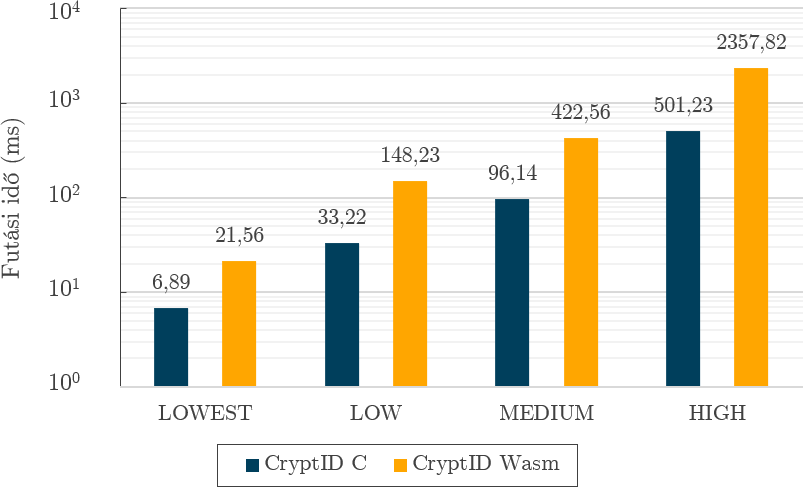
\includegraphics[height=225px]{05-cryptid/tate-pairing-chart.png}
    \caption{A Tate párosítás futási ideje.}
    \label{Figure::CryptID::TatePairingChart}
\end{figure}

Az \dotref{Figure::CryptID::TatePairingChart} ábra logaritmikus skálára vetítve mutatja a Tate párosítás különböző nagyságú bemeneteken mért futási idejét. Itt szeretnénk felhívni a figyelmet arra, hogy a grafikonon szereplő adatok ezúttal milliszekundumban kerültek rögzítésre. Az egyes sávok fölött található értékekből könnyen kiszámolható, hogy a WebAssembly bináris megközelítőleg háromszor-ötször tovább fut, mint a natív kód. A különbség tehát a skaláris szorzásnál mérthez hasonló.

Önmagában az ilyen mértékű sebességkülönbség jelenléte kellemetlennek tekinthető, azonban az eltérés konzisztens volta fontos bizonyíték arra vonatkozóan, hogy a WebAssembly környezet teljesítménye stabil, nem ingadozik.

\paragraph{Optimalizációs lehetőségek}

Az optimalizációra a Tate párosítás esetén két út kínálkozik: hatékonyabb algoritmus implementálása, illetve a meglevő algoritmus által hívott rutinok javítása. A következőkben az utóbbi lehetőséget tekintjük, azonban későbbi munkánk során szeretnénk algoritmikus módosításokat is megvizsgálni.

Az \dotref{Figure::CryptID::EncryptProfileChart} ábrán az \textit{Encrypt} teljesítményét meghatározó két függvény, a \texttt{TatePairing} \linebreak és a \texttt{HashToPoint} futási ideje szerepel egy \texttt{HIGH} bemenetre. A diagramon szereplő adatokból leolvasható, hogy a Tate párosítás teljesítménye mindenekelőtt a modulo hatványozást végző \texttt{modPow} és a multiplikatív inverzt számító \texttt{mulInv} futási idejének függvénye.

Úgy gondoljuk, hogy mindkét függvény teljesítményében jelentős előrelépés érhető el mikrooptimalizációk alkalmazásával. Ez a processzor \textit{cache} jobb kihasználását, a függvényhívások számának minimalizálását, valamint a függvényparaméterek és visszatérési értékek hatékonyabb kezelését foglalhatja például magában.

\subsection{Identity-based Encryption}

A két legfontosabb alaprutin áttekintése után következhet az Identity-based Encryptiont alkotó függvények (\textit{Setup, Encrypt, Extract, Decrypt}) teljesítményének elemzése. Tekintve, hogy a \textit{Setup} és az \textit{Extract} inkább szerveroldalon kerülhet felhasználásra, ezek esetében csupán a natív C és a Node.js-ben futtatott Wasm verziót hasonlítottuk össze. Az \textit{Encrypt} és a \textit{Decrypt} futási idejét azonban ezeken felül egy asztali és egy mobilos böngészőben is megmértük.

\subsubsection{Setup}

A \textit{Setup} függvény segítségével új publikus paramétereket és mesterkulcsot állíthatunk elő. Ezek generálása nem tekinthető olyan gyakori tevékenységnek, mint a titkosítás, a visszafejtés vagy a privát kulcs kinyerés. Ennélfogva a \textit{Setup} teljesítményével szemben támasztott elvárásaink kevésbé voltak szigorúak.

\begin{figure}[h]
    \centering
    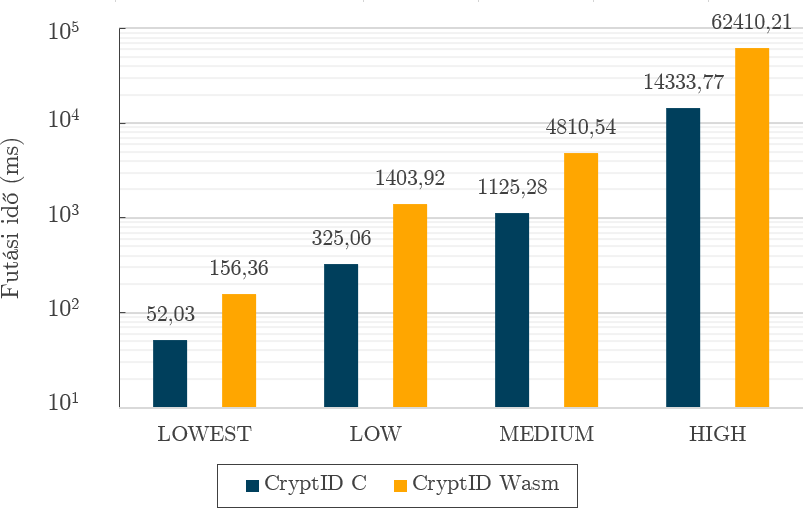
\includegraphics[height=225px]{05-cryptid/setup-chart.png}
    \caption{A \textit{Setup} függvény futási ideje.}
    \label{Figure::CryptID::SetupChart}
\end{figure}

A \textit{Setup} különböző nagyságú bemeneteken mért futási idejét az \dotref{Figure::CryptID::SetupChart} ábrán láthatjuk. Az egyes futási idők már egészen más nagyságrendben mozognak, mint például a skaláris szorzás esetén: a WebAssembly verzió \texttt{HIGH} bementre már több mint egy percig futott! Mi több, ugyanezen bemeneten a C változat is megközelítőleg $15$ másodpercig dolgozott.

\paragraph{Optimalizációs lehetőségek}

A \textit{Setup} teljesítményét a megfelelő értékek generálása határozza meg. Ennek folytán a futási idő javítható a generálási folyamat optimalizálásával, vagy a generált értékek számának csökkentésével. Utóbbi megoldás minimális befektetéssel kínál nagyságrenddekkel jobb teljesítményt, emiatt például a MIRACL is rögzít bizonyos elliptikus görbe paramétereket. Úgy gondoljuk, hogy ez a CryptID számára is megfelelő előrelépési lehetőség lenne, azonban még meg kell határoznunk azokat az értékeket, melyeket a kódban rögzíthetünk.

\subsubsection{Extract}

Az \textit{Extract} függvény a privát kulcsok kinyerésére szolgál. Ezt a feladatot a PKG végzi, aminek következtében \textit{Setuphoz} hasonlóan az \textit{Extract} esetén is elsősorban szerveroldali felhasználással számoltunk. Alapvető eltérés ugyanakkor, hogy az \textit{Extract} végrehajtási gyakorisága előreláthatólag jóval meghaladja a \textit{Setupnál} feltételezhetőt. Ennek folytán a futási ideje is kellőképpen alacsony kell, hogy legyen. 

\begin{figure}[h]
    \centering
    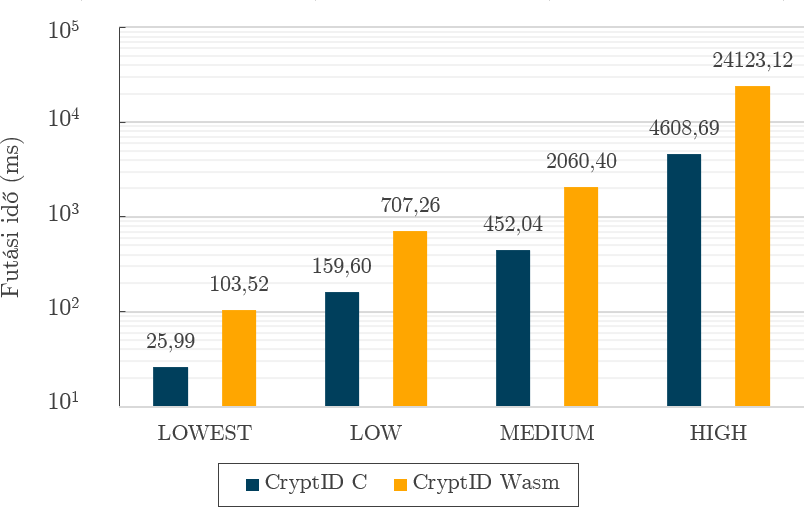
\includegraphics[height=225px]{05-cryptid/extract-chart.png}
    \caption{Az \textit{Extract} függvény futási ideje.}
    \label{Figure::CryptID::ExtractChart}
\end{figure}

Az \dotref{Figure::CryptID::ExtractChart} ábra a \textit{Extract} függvény futási idejét jeleníti meg. Míg a \texttt{LOWEST}, a \texttt{LOW} és a \texttt{MEDIUM} bemenetek esetén kielégítő értékekről beszélhetünk még a WebAssembly binárist tekintve is (legfeljebb $2$ másodperc), addig a \texttt{HIGH} bemenethez tartozó eredmények már meghaladják a kívánatosnak gondolt $1$–$2$ másodperces határt. A Wasm verzió különösen rossz, mintegy $24$ másodperces eredménnyel rendelkezik.

\paragraph{Optimalizációs lehetőségek}

Az \textit{Extract} futási idejét befolyásoló egyetlen komponens a \texttt{HashToPoint} eljárás. Az \dotref{Figure::CryptID::EncryptProfileChart} ábráról leolvasható, hogy ennek teljesítményét a skaláris szorzást megvalósító \texttt{affineMul} dominálja. Ez azt jelenti, hogy az \textit{Extract} futási idejét a skaláris szorzás felgyorsításával tudjuk javítani.

\subsubsection{Encrypt}

A titkosítást megvalósító \textit{Encrypt} függvény futását már egy asztali, valamint egy mobilos böngészőben is lemértük. Ennek oka, hogy a titkosítás kifejezetten egy kliensoldali műveletnek tekinthető, és ennek megfelelően legtöbbször a böngészőben kerül majd végrehajtásra. A hatékony implementáció ezúttal kiemelt fontosságot nyer, hiszen a mobil eszközök csak korlátozott erőforrásokkal rendelkeznek.

\begin{figure}[h]
    \centering
    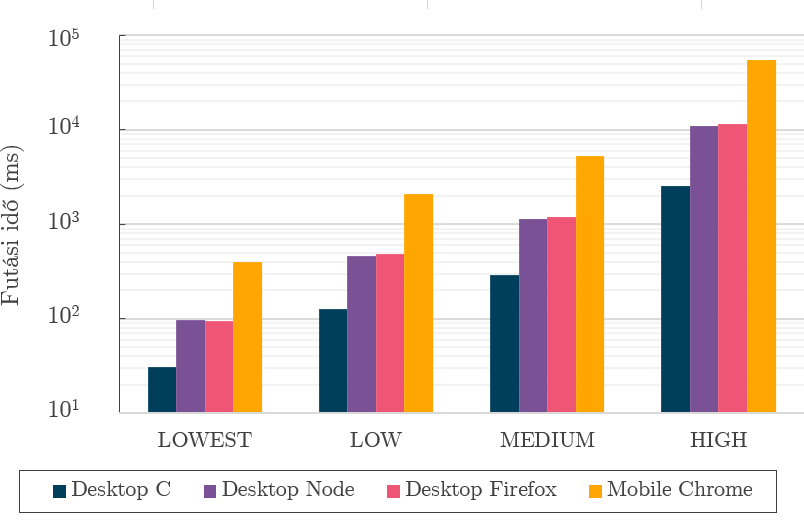
\includegraphics[height=225px]{05-cryptid/encrypt-chart.png}
    \caption{Az \textit{Encrypt} függvény futási ideje.}
    \label{Figure::CryptID::EncryptChart}
\end{figure}

A \dotref{Figure::CryptID::EncryptChart} ábrán ismét megfigyelhető a már látott tendencia: a Node.js-alapú WebAssembly háromszor-négyszer nagyobb értékeket produkál, mint a natív kód. Megjelenik emellett az asztali Firefox böngésző, mely nagy meglepetésünkre a Node.js-szel megegyező idők alatt futtatja a függvényt. Ez számunkra egy váratlan fordulat volt, hiszen előzetesen azt vártuk, hogy a böngésző, mint összetettebb beágyazó környezet, a Node.js-nél alacsonyabb teljesítményt fog biztosítani.

Sajnos a mobilos böngészőben történő végrehajtás jelentősen leszakad a többi értéktől: mintegy négyszer-ötször lassabb, mint az asztali WebAssembly. Ennek hátterében természetesen az architekturális, valamint erőforrásbeli különbségeket érdemes keresnünk.

\paragraph{Optimalizációs lehetőségek}

A könyvtárt integráló alkalmazások felhasználói élményét jelentősen befolyásolja a két legtöbbet használt függvény, az \textit{Encrypt} és a \textit{Decrypt} futási ideje. Ennek folytán kiemelt figyelemmel érdemes kezelni az ezekben adódó optimalizációs lehetőségeket.

A \dotref{Figure::CryptID::EncryptProfileChart} ábrán az \textit{Encrypt} egy futása során gyűjtött adatokat láthatunk. A bal oldali kördiagram az \textit{Encrypt} által hívott függvények végrehajtási idejét ábrázolja a teljes futási időhöz képest. Erről egyértelműen leolvasható, hogy a teljesítményt a \texttt{TatePairing} és a \texttt{HashToPoint} eljárás határozza meg. Ezen függvények összetevőit a jobb oldali kördiagramok ábrázolják.

Az \textit{Encrypt} sebessége tehát a Tate párosításnál ismertetett módszerek segítségével, valamint a \texttt{HashToPoint} függvényben szerepet játszó skaláris szorzás felgyorsításával növelhető.

\begin{figure}[h]
    \centering
    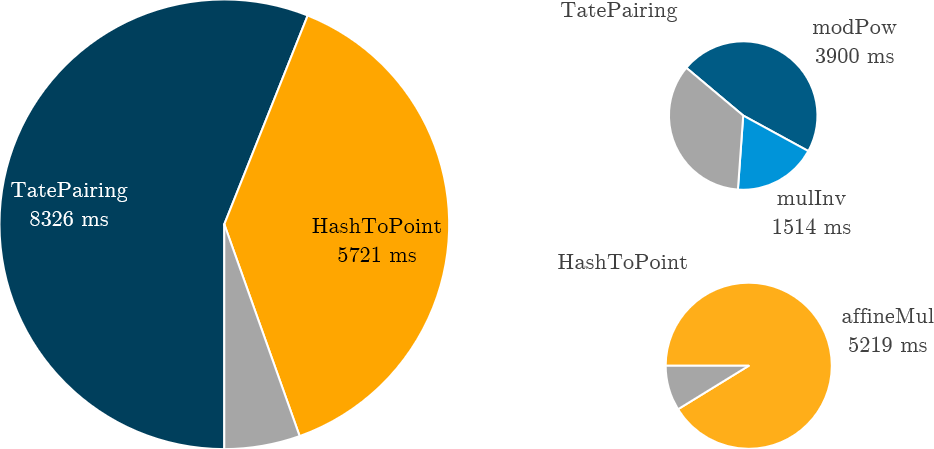
\includegraphics[height=210px]{05-cryptid/encrypt-profile-chart.png}
    \caption{Az \textit{Encrypt} függvényt alkotó komponensek futási ideje egy \texttt{HIGH} bemenetre (Desktop Firefox környezet).}
    \label{Figure::CryptID::EncryptProfileChart}
\end{figure}

\subsubsection{Decrypt}

Az \textit{Encrypthez} hasonlóan a \textit{Decrypt} futási idejét is négy környezetben mértük. Elvárásainkat az előző mérések vezérelték: úgy gondoltuk, hogy a natív C változat lesz a leggyorsabb, azonos időt ad a Desktop Node.js és a Firefox, a sort pedig a mobilos Chrome zárja. 

\begin{figure}[h]
    \centering
    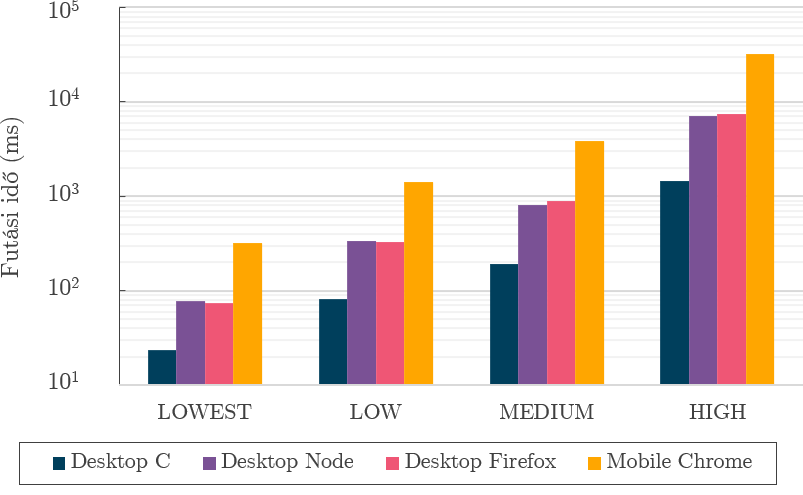
\includegraphics[height=225px]{05-cryptid/decrypt-chart.png}
    \caption{A \textit{Decrypt} függvény futási ideje.}
    \label{Figure::CryptID::DecryptChart}
\end{figure}

Az \dotref{Figure::CryptID::DecryptChart} ábráról leolvasható adatok pontosan az említett elvárásokat igazolják: az \textit{Encryptnél} látott relatív különbségek jelennek meg itt is. Felfedezhető a hasonlóság mindamellett az abszolút futási időt tekintve is: a \textit{Decrypt} végrehajtási ideje megközelítőleg $\frac{2}{3}$-a az \textit{Encryptének}. Ez a párhuzam abból adódik, hogy a \textit{Decrypt} sebességét szinte kizárólag a \texttt{TatePairing} határozza meg, \texttt{HashToPoint} hívás viszont ezúttal nincsen. 

\paragraph{Optimalizációs lehetőségek}

A \textit{Decrypt} teljesítményét a Tate párosítás dominálja, így ennek javítása tekinthető a legígéretesebb optimalizációs lehetőségnek.

\subsection{Összegzés}

A CryptID alapjául szolgáló legfontosabb rutinok teljesítményét látva kijelenthető, hogy asztali környezetben a könyvtár használhatónak tekinthető még nagyobb bemenet esetén is, mobil eszközökön azonban csak kisebb bemenetekre várhatunk kielégítő végrehajtási időt. Érdemes azonban ezen értékeléshez hozzátenni, hogy ezt a teljesítményt a CryptID javarészt egyszerűbb algoritmusok kevésbé hatékony megvalósításaival éri el. Emiatt számos, az előzőekben is felsorolt optimalizációs lehetőség adódik, melyek alkalmazásával a könyvtár teljesítménye jelentősen növelhető, megfelelő futási időt nyújtva mobil eszközökön is.

    \chapter{Alkalmazások}
\label{Chapter::Alkalmazasok}

Az \dotref{Section::CryptID::ApplicationDevelopment} alfejezet API-használatra fókuszáló példaprogramja után ebben a fejezetben nagyobb léptékű alkalmazásokat mutatunk be. A fejezet célja, hogy valós, gyakorlati példákat adjon olyan webalkalmazásokra, melyek kulcsösszetevője lehet az IBE, s ezáltal a CryptID.

Előbb egy ténylegesen implementált webalkalmazást – CrpytID.email – ismertetünk, majd Személyre szabott zárthelyi néven egy rövid esettanulmány formájában vázoljuk az IBE egy lehetséges egyetemi felhasználását.

\section{Implementáció – CryptID.email}

A CryptID.email egy fájltitkosításra szolgáló platformfüggetlen webalkalmazás, melynek legfontosabb jellemzői a következők:

\begin{outdentlist}
    \item[]\textbf{Email, mint azonosító.}
    Az IBE-t használó alkalmazások implementációjában kulcsfontosságú kérdés, hogy mit használjunk azonosítóként. Míg egy vállalati belső alkalmazás esetén ez a legtöbbször adott (például LDAP útján), addig egy nyílt, tetszőleges felhasználó által igénybe vehető szolgáltatás esetén ez korántsem egyértelmű.
    
    Az azonosító kiválasztásának két kiemelkedő szempontja az azonosító elterjedtsége (hány felhasználó rendelkezik vele?) valamint ellenőrizhetősége (mennyire bonyolult ellenőrizni, hogy egy azonosító valóban egy adott entitáshoz tartozik?). Ezek figyelembevételével a CrpytID.email esetén az email címet választottuk azonosítóként, hiszen az internetfelhasználók zöme rendelkezik legalább egy email címmel, valamint ellenőrizni is egyszerűbb, mint egy telefonszámot vagy egy Facebook-hozzáférést.

    \item[]\textbf{Szimmetrikus tartalomtitkosítás.}
    Az aszimmetrikus módszerek (mint az IBE) alacsony teljesítményük miatt nem alkalmasak nagyobb adattömeg titkosítására. Emiatt gyakori megoldás, hogy az aszimmetrikus kriptográfiát egy nagyságrendekkel gyorsabb szimmetrikus módszer kulcsának titkosítására használják. 

    Ezen ötlet jelenik meg a CryptID.email implementációjában is: Először generálunk egy véletlenszerű bájtsorozatot, mely a fájlok tartalmának titkosításához használt AES (\textit{Advanced Encryption Standard}) eljárás kulcsa lesz. Az AES titkosítás végeztével pedig az említett kulcsot a CryptID könyvtárral aszimmmetrikusan titkosítjuk.

    Ennek köszönhetően egyszerre élvezhetjük az IBE nyújtotta előnyöket, valamint a szimmetrikus titkosítás gyorsaságát.

    \item[]\textbf{Kliensoldali titkosítás.}
    Az IBE meghatározó jellemzője, hogy a visszafejtésre alkalmas privát kulcsokat egy megbízható fél, a PKG generálja. Ez azonban azt is jelenti, hogy a PKG tetszőleges publikus kulcshoz képes privát kulcsot előállítani. Ugyanakkor ez a lehetőség csak akkor jelent kockázatot, ha a PKG (vagy valamely, azzal közvetlen kapcsolatban álló komponens) a publikus kulcson kívül az azzal titkosított adatokhoz is hozzáfér.

    Ennek elkerülésére a CryptID.email kliensoldali titkosítást valósít meg, azaz mind a titkosítás, mind a visszafejtés úgy történik, hogy a publikus kulcson kívül semmilyen adat nem hagyja el a felhasználó eszközét.

\end{outdentlist}

A következőkben a titkosítás, majd a visszafejtés lépésein keresztül ismertetjük az alkalmazás megvalósításának részleteit.

\subsection{Titkosítás}

\subsubsection{A fájl beolvasása}

A titkosítási folyamat első lépése – természetesen a megfelelő webhely felkeresését követően – a titkosítandó fájl beolvasása. Ez a fájl teljes tartalmának memóriába történő beolvasását jelenti. Ugyan a CryptID.email által használt FileReader API\footnote{\url{https://w3c.github.io/FileAPI/#dfn-filereader} – \url{https://caniuse.com/#feat=filereader}} lehetővé teszi, hogy egyszerre csak a fájl egy kisebb szeletét olvassuk be és dolgozzuk fel (azaz \textit{streameljük}), azonban a böngészők jelenleg nem biztosítanak hatékony \textit{streaming} titkosítási eljárásokat, így ennek megfelelő kihasználása nem lehetséges.

\subsubsection{A fájl tartalmának titkosítása}

Miután a memóriában rendelkezésre áll a titkosítandó adat, a CryptID.email a WebCrypto API-n\footnote{\url{https://www.w3.org/TR/WebCryptoAPI/} – \url{https://caniuse.com/#feat=cryptography}} keresztül előbb generál egy AES kulcsot, majd ugyanezen API-t használva AES-GCM (\textit{Galois/Counter Mode}) blokktitkosítással rejtjelezi a bemenetet.

Ezzel a memóriában már készen áll egy szimmetrikus privát kulcs, valamint az ezzel titkosított adattömeg.

\subsubsection{Címzett kiválasztása}

Az IBE titkosítás megkezdése előtt a felhasználónak meg kell adnia a címzett email címét, ami a publikus kulcsban szereplő azonosítót jelenti.

\subsubsection{Publikus paraméterek lekérése}

A szimmetrikus kulcs titkosítása előtt szükséges a publikus IBE paraméterek beszerzése. Ezeket a szerver szolgáltatja, mely a paramétereken felül egy azokhoz köthető azonosítót is elküld a kliensnek. Erre azért van szükség, mert a szerver havonta új publikus paramétereket és mesterkulcsot generál (a \texttt{CryptID.setup} függvényt igénybe véve), viszont a korábban titkosított adatok feloldására ezek természetesen nem alkalmasak, így tárolni és azonosítani kell őket.

\subsubsection{A szimmetrikus kulcs titkosítása}

A következő lépés a fájl tartalmának rejtjelezéséhez használt szimmetrikus kulcs titkosítása. Ez a CryptID könyvtár \texttt{encrypt} függvényén keresztül történik, az előző lépés során megszerzett publikus paraméterek és az email címből képzett publikus kulcs segítségével.

\subsubsection{A titkos fájl összeállítása}

A CryptID.email a titkosított tartalmat nem juttatja el a címzetthez – arról a felhasználónak kell gondoskodnia. Ennek elősegítésére a CryptID.email létrehoz egy titkos fájlt, mely a következő összetevőket foglalja magában:

\begin{outdentlist}
    \item[]\textbf{Eredeti fájlnév.}
    A titkosított fájlhoz tartozó eredeti fájlnévre elsősorban a kiterjesztés megőrzése miatt van szükség, mely számos operációs rendszeren kitüntetett jelentéssel bír.

    \item[]\textbf{Publikus paraméterek.}
    A szimmetrikus kulcs titkosításához felhasznált publikus IBE paraméterek azonosítója. A CryptID.email szerveroldali komponense ez alapján tudja megkeresni a privát kulcs generálásához szükség mesterkulcsot.

    \item[]\textbf{Titkosított szimmetrikus kulcs.}
    Az IBE-titkosított AES kulcs.

    \item[]\textbf{Titkosított fájltartalom.} 
    Az eredeti fájl tartalma AES-titkosítva.
\end{outdentlist}

A titkos fájlt ezután a felhasználó a memóriából a háttértárra mentheti, majd igény szerint továbbíthatja.

\subsection{Visszafejtés}

A visszafejtés lépéssora ott veszi fel a fonalat, hogy a felhasználó valamilyen módon hozzájutott egy, a CryptID.emailen keresztül előállított titkos fájlhoz, és szeretné visszafejteni az ebben tartalmazott eredeti fájlt. A visszafejtés azonban csak egy megfelelő privát kulcs birtokában sikerülhet. A privát kulcs beszerzésehez pedig a felhasználónak egy azonosítási folyamaton keresztül igazolnia kell az email címét.

Tekintve, hogy a visszafejtési folyamat a titkosítás inverze, megjelennek hasonló lépések, mint például a fájl memóriába olvasása. Ezek részletes ismertetését itt elhagyjuk, és csak a lényeges pontokat mutatjuk be részletesen.

\subsubsection{Email cím megadása}

Az azonosítási folyamat elindításához a felhasználónak először meg kell adnia az email címét a CryptID.email weboldalán.

\subsubsection{Megerősítő email kiküldése}

A CryptID.email szerveroldali komponense ezután generál egy nyolc karakter hosszúságú, úgynevezett email tokent, melyet SendGriden\footnote{\url{https://sendgrid.com/}} keresztül kiküld a felhasználó által megadott email címre. A token csupán tíz percig érvényes, ezt követően nem alkalmas az email cím igazolására.

\subsubsection{Email token megadása}

Ha a megadott email cím valóban a felhasználó tulajdonában áll, akkor megkapja az említett email tokent is, melyet aztán megadhat a CryptID.email weboldalán. Ezzel a felhasználó igazolta az identitását, elindulhat a privát kulcs kinyerése.

\subsubsection{Privát kulcs generálás}

Az identitás ellenőrzését követően a szerver meghatározza a fájl titkosítása során használt publikus paramétereket, valamint a privát kulcs generálásához szükséges mesterkulcsot a titkos fájlban tárolt azonosítón keresztül.  Ezeket a korábban megadott email cím mellett továbbítja a PKG felé, mely a \texttt{CryptID.extract} függvényt meghívva előállítja a publikus kulcs privát párját. Végül a szerver a privát kulcsot elküldi a kliensnek.

\subsubsection{A szimmetrikus kulcs visszafejtése}

A privát kulcs birtokában a kliens megpróbálkozhat a titkos fájlban tárolt szimmetrikus kulcs visszafejtésével. Ehhez a kliens a CrpytID könyvtár \texttt{decrypt} függvényét használja. Amennyiben a privát kulcs helyes, azaz valóban a szóban forgó felhasználó email címével titkosították a szimmetrikus kulcsot, akkor a visszafejtés sikeres lesz. Ellenkező esetben a folyamat itt megáll, a felhasználó nem fér hozzá az eredeti tartalomhoz.

\subsubsection{Az eredeti fájl visszaállítása}

A folyamat utolsó lépése az eredeti fájl tartalmának visszafejtése, mely az előzőleg nyert szimmetrikus kulcs és a WebCrypto API segítségével történik. A memóriában előálló nyílt reprezentációt ezután a felhasználó a háttértárra mentheti. A visszafejtési folyamat ezzel véget ért, visszaállítottuk az eredeti fájlt.

\subsection{Összegzés}

A CryptID.email különböző eszközökön és platformokon átívelő egységes titkosítási megoldást nyújt. A használatához nem szükséges sem előzetes kulcscsere, sem a PKI (\textit{public key infrastructure}) használata, hiszen a továbbítandó fájlok titkosításához csupán a címzett email címét kell megadnunk.


\section{Esettanulmány – Személyre szabott zárthelyi}
\label{Section::Applications::Zarthelyi}

Míg az előző alkalmazás a CryptID hordozható és könnyen használható voltát demonstrálta, addig a személyre szabott zárthelyit leíró rövid esettanulmány elsődleges célja a metaadatok beágyazásának bemutatása. Tapasztalataink szerint a metaadatok leginkább egy adott szakterületen belül lehetnek hasznosak, ezért kézenfekvő választás volt az esettanulmány témájának az általunk jól ismert zárthelyi dolgozatok világa.

Az alkalmazás hallgatónként egyedi elektronikus feladatsorok összeállítását teszi lehetővé, melyek a titkosításnak köszönhetően akár napokkal a dolgozat időpontja előtt elhelyezhetők az egyetemi számítógépeken.

\subsection{Motiváció}

A motiváció a csalások megelőzésében gyökerezik: úgy gondoljuk, hogy a hálózati hozzáférés korlátozásával szemben sokkal hatásosabb eszközt jelent a visszaélések megakadályozásában, ha minden hallgató eltérő feladatsorral rendelkezik. Ennek kezelése azonban a különböző feladatsorok előállításán és ellenőrzésén felül további problémákat is felvet. Ahhoz, hogy ez az elképzelés valóban csökkentse a csalások számát, biztosítani kell, hogy minden hallgató csak a saját feladatsorához férjen hozzá és csak a zárthelyi időpontjában. 

Úgy gondoltuk, hogy erre a célra a CryptID biztosította IBE egy valódi megoldást nyújthat.

\subsection{Megvalósítás}

A rendszer elméleti megvalósítását a publikus kulcs megtervezésén keresztül mutatjuk be. A következőkben egyenként hozzáadunk három mezőt a publikus kulcshoz, kifejtve egyúttal az adott mező implementációval való kapcsolatát. A publikus kulcs tartalmának ilyen módon történő leírása teret enged az alkalmazás összes fontos aspektusának bemutatására.

\subsubsection{Neptun-kód}

A publikus kulcs nélkülözhetetlen összetevője egy, a hallgatók azonosítására szolgáló mező. Természetes választás a Neptun-kód, mellyel Karunk minden hallgatója rendelkezik. Előnyös tulajdonsága továbbá, hogy ellenőrzése már kiépített infrastruktúrán keresztül megtehető: a privát kulcs generálása előtt a hallgató a hálózati azonosítóját használva bejelentkezik, ezzel igazolva az identitását.

Önmagában mindazonáltal a Neptun-kód nem elégséges. Ha a feladatsort csak a címzett hallgató azonosítójával titkosítjuk, akkor a visszafejtéshez használt privát kulcs tetszőleges, a hallgatónak szánt feladatsor visszafejtésére alkalmas lesz!

\subsubsection{Dátum}

Érdemes tehát az előbb említett probléma megakadályozására egy újabb mezővel, a dátummal kiegészíteni a publikus kulcsot. Titkosításkor a Neptun-kód mellett a zárthelyi dolgozat dátumát is felhasználjuk, a privát kulcs generálása előtt pedig a rendszer automatikusan elhelyezi az aktuális dátumot a publikus kulcsban. Ez rendkívül egyszerűen megtehető, hiszen csak egy JSON objektumot kell egy újabb mezővel kiegészíteni.

Gondot jelenthet ugyanakkor, amennyiben a hallgató egy napon több zárthelyit is ír. Erre egy lehetséges válasz a publikus kulcsban elhelyezett dátum finomságának növelése, például \textit{év-hónap-nap} helyett \textit{év-hónap-nap-óra} mezők használatával. Jobb megoldást kínál azonban a publikus kulcs további bővítése.

\subsubsection{Tárgy}

A bővítés ötlete azon alapszik, hogy a titkosításhoz felhasználhatjuk a szóban forgó tárgy nevét is. Nem szabad azonban elfelejteni, hogy csak olyan mezőt érdemes elhelyeznünk a publikus kulcsban, melyet aztán a privát kulcs generálásakor ellenőrizni tudunk.

A \textit{tárgy} mezőt ezért a dátumhoz hasonlóan közvetlenül a szerveroldalon helyezzük el a publikus kulcsban, a privát kulcs generálása előtt, megkerülve ezzel az ellenőrzés szükségességét. Ekkor azonban biztosítani kell, hogy a mező értéke megbízható forrásból származzék. Ehhez a hallgató által a zárthelyi megírásához használt számítógép IP címe nyújthat alapot. Ha az IP cím alapján meghatározható a terem, ahol az eszköz elhelyezkedik, akkor ezt az információt a teremfoglalási adatbázissal összekapcsolva egyértelműen meg tudjuk mondani, hogy a hallgató épp milyen tárgyhoz kötődő zárthelyin vesz részt.

Ez a mező tehát a fizikai hely közvetett ellenőrzésének lehetőségét nyújtja.

\subsection{Összegzés}

A vázolt alkalmazás garantálja, hogy az egyes feladatsorok visszafejtése csak a kívánt hallgató által, a kívánt időben és helyen végezhető el. Mindezen követelmények kikényszerítése automatikusan, a publikus kulcsban elhelyezett metaadatok segítségével történik.

Ennek köszönhetően a dolgozatokhoz használt feladatsorok jóval a zárthelyi tényleges időpontja előtt elhelyezhetők a számítógépeken, valamint akár hálózati korlátozás is alkalmazható – csupán a PKG-hez történő hozzáférést kell biztosítani.

Mindamellett nem szabad elfelejtkeznünk arról, hogy CryptID alternatívája lehet az egyszerű szimmetrikus titkosítás alkalmazása: a feladatsorok előállításával egy időben minden feladatsorhoz generálunk egy szimmetrikus kulcsot, melyhez a hallgató csak sikeres azonosítás után férhet hozzá. Csakhogy az IBE egyik lehetséges alkalmazási területét épp az ilyen, sok szimmetrikus kulcs menedzselését igénylő rendszerek kiváltása jelenti, hiszen a mesterkulcson felül semmilyen más kulcs tárolására nincsen szükség.

    \chapter{Összefoglalás}

A dolgozatunkban a Boneh-Franklin IBE egy újszerű megvalósítását mutattuk be, előbb a matematikai alapokat, aztán az implementáció részleteit kifejtve. Az elkészült könyvtár célja, hogy az elérhető megvalósítások valós alternatívája legyen, egyedi jellemzőinek köszönhetően.

\section{A CryptID jellemzői}

A CryptID újdonságtartalommal bíró sajátosságai két irányból is megközelíthetők, előbb a technológiai alapokat, majd az IBE rendszert tekintve. A könyvtár egyedülálló karakterisztikája a hordozhatóság: a WebAssembly biztosította platformfüggetlenségre építve asztali, mobil és IoT eszközökön is elérhető titkosítási szolgáltatást nyújt. A hordozhatóság egyszerű integrálhatósággal párosul, mely megkönnyíti a dolgozatban ismertetetthez hasonló webes vagy asztali alkalmazások elkészítését.

Hangsúlyos a publikus kulcs szerepe is: az IBE egyedülálló tulajdonsága, hogy a publikus kulcs valójában egy azonosító; ezt bővíti ki a CryptID metaadatok hozzáadásal, ráadásul mindezt strukturált, könnyen kezelhető formában. Ez egészen új szakterület-specifikus alkalmazások előtt nyitja meg az utat, melyre egy szemléletes példa a \dotref{Section::Applications::Zarthelyi} alfejezetben bemutatott személyre szabott zárthelyi.

A funkcionalitás mellett nagy figyelmet fordítottunk az implementáció megfelelő teljesítményére is, hiszen a kriptográfiai programkönyvtárak összehasonlításának egyik kiemelt szempontja a különböző erőforrásokkal (memória, processzoridő) való hatékony gazdálkodás. Ez még hangsúlyosabb szerepet nyer, ha a korlátozott erőforrásokkal rendelkező mobil eszközöket tekintjük. A \dotref{Section::Performance} alfejezetben elemzett mérések tanúsága szerint a CryptID kielégítő futási idővel rendelkezik asztali és mobil eszközökön is.

\section{Továbblépési lehetőségek}

A könyvtár további fejlesztése számos irányban folytatható. Kiemelkedik ezek közül azonban a korábban részletezett optimalizációk által kijelölt irány, melynek mentén a CryptID futási ideje nagyságrendekkel csökkenthető. Ilyen például a Heuberger-Mazzoli elliptikus skaláris szorzás, a rögzített paraméterek használata, vagy a hatékonyabb Tate párosítás alkalmazása. Ezen felül teljesítménynövekedést érhetünk el különböző mikrooptimalizációk segítségével is.

Nemcsak a futási idő, hanem a bináris méretének csökkentése is fontos szempont, hiszen ezzel mérsékelhető a hálózati adatforgalom nagysága. Tekintve, hogy a CryptID méretének jelentős részét a külső könyvtárak (GMP, OpenSSL) teszik ki, így szeretnénk megvizsgálni ezek eltávolításának, kiváltásának vagy tömörítésének lehetőségét. Utóbbira hatékony megoldást jelenthet például az úgynevezett \textit{tree-shaking}, mely a nem használt kódrészletek eldobását jelenti.

Annak érdekében, hogy a CryptID valós alkalmazások alapját szolgáltathassa, növelnünk kell az ismertségét, melyet különböző konferenciákon történő részvétellel szeretnénk elősegíteni. Ezek egyúttal kiváló alkalmat kínálnak a visszajelzések, fejlesztési lehetőségek gyűjtésére is.

A titkosításon túl további azonosító alapú rendszerek is léteznek, amelyek magja rendkívül hasonló. Ilyenek például az Identity-based Signature \cite{Yi::IBS} és Identity-based Cloud Authentication Protocol \cite{Huszti::IdentityBasedCloudAuthentication}. A hasonlóság miatt megfontolandó az efféle rendszerek implementációja is, hiszen a CryptID magában hordoz számos olyan réteget, amelyek a további sémák fejlesztése során módosítás nélkül vagy kis módosítással újrahasználhatók.


    \bibliography{references.bib}

    \chapter*{Függelék}
\addcontentsline{toc}{chapter}{Függelék}
% Ez majd még máshogy lesz, de egyelőre így volt a legegyszerűbb

\section*{CryptID – WebIDL definíciók}
\addcontentsline{toc}{section}{CryptID – WebIDL definíciók}

\lstinputlisting[language=WebIDL]{./code/cryptid.webidl}

\pagebreak

\section*{CryptID – Példaprogram}
\addcontentsline{toc}{section}{CryptID – Példaprogram}

\lstinputlisting[language=JavaScript, escapechar=^, showstringspaces=false]{./code/application-development-with-cryptid.js}

\pagebreak

\section*{CryptID – Teljesítmény}
\addcontentsline{toc}{section}{CryptID – Teljesítmény}

\subsection*{A mérésekhez használt környezetek}

\begin{table}[h!]
\captionsetup{justification=centering}
\centering
  \begin{tabular}{|| l | c ||}
  \hline
  Paraméter & Érték \\
  \hline \hline
  Típus        & Dell Inspiron 5567 (2017) \\
  Processzor   & i7-7500U, 2,7 GHz \\
  Memória      & 16 GB, DDR4, 2133 MHz \\
  \hline
  \end{tabular}
\caption{Desktop hardverkonfiguráció.}  
\label{Fuggelek::Table::BenchmarkDesktopHardware}
\end{table}

\begin{table}[h!]
\captionsetup{justification=centering}
\centering
  \begin{tabular}{|| l | c ||}
  \hline
  Szoftver & Verzió \\
  \hline \hline
  Operációs rendszer & Ubuntu 16.04.4 LTS \\
  \hline
  emscripten & 1.38.8 \\
  gcc & 5.4.0 20160609 \\
  Node.js & v8.9.1 \\
  \hline
  \end{tabular}
\caption{Desktop natív és Node.js szoftverkonfiguráció.}  
\label{Fuggelek::Table::BenchmarkDesktopNativeSoftware}
\end{table}

\begin{table}[h!]
\captionsetup{justification=centering}
\centering
  \begin{tabular}{|| l | c ||}
  \hline
  Szoftver & Verzió \\
  \hline \hline
  Operációs rendszer & Windows 10 Education, Version 1803 (OS Build 17134.35) \\
  \hline
  Firefox Quantum & 62.0.3 \\
  \hline
  \end{tabular}
\caption{Desktop Firefox szoftverkonfiguráció.}  
\label{Fuggelek::Table::BenchmarkDesktopFirefoxSoftware}
\end{table}

\begin{table}[h!]
\captionsetup{justification=centering}
\centering
  \begin{tabular}{|| l | c ||}
  \hline
  Paraméter & Érték \\
  \hline \hline
  Típus        & Nokia 6.1 TA-1043 \\
  Processzor   & Qualcomm Snapdragon 630, 2.2 GHz \\
  Memória      & 3 GB, LPDDR4, 1333 MHz \\
  \hline
  \end{tabular}
\caption{Mobil hardverkonfiguráció.}  
\label{Fuggelek::Table::BenchmarkMobileHardware}
\end{table}

\begin{table}[H]
\captionsetup{justification=centering}
\centering
  \begin{tabular}{|| l | c ||}
  \hline
  Szoftver & Verzió \\
   \hline \hline
  Operációs rendszer & Android 8.1.0 - Kernel 4.4.78-perf+ \\
  \hline
  Chrome for Mobile & 68.0.3440.91 \\
  \hline
  \end{tabular}
\caption{Mobil szoftverkonfiguráció.}  
\label{Fuggelek::Table::BenchmarkMobileSoftware}
\end{table}

\begin{table}[H]
\captionsetup{justification=centering}
\centering
  \begin{tabular}{|| l | c ||}
  \hline
  Könyvtár & Verzió \\
  \hline \hline
  libpari-dev                        & 2.11.0-1 \\
  \hline
  MIRACL                  & commit 4bd13901519d329c6c1369fb3322b52fe10c7a6e\footnote{\url{https://github.com/miracl/MIRACL}} \\
  \hline
  \end{tabular}
\caption{A felhasznált könyvtárak verziói.}  
\label{Fuggelek::Table::BenchmarkLibraries}
\end{table}

\subsection*{Mérési metodológia}

A teljesítménymérésekhez minden platformon a Google Benchmark\footnote{\url{https://github.com/google/benchmark}, verzió: commit af441fc1143e33e539ceec4df67c2d95ac2bf5f8} könyvtárat használtuk. 

Egy teszt egy adott függvény adott bementre történő $n$ egymást követő lefuttatását jelenti (ezeket iterációknak nevezzük), ahol $n$ értékét a Benchmark könyvtár határozza meg a függvény sebességének megfelelően. A teszt eredménye az iterációk során mért idők átlaga.

Az egyes függvényekhez rendelt végleges időket függvényenként húsz, a fentieknek megfelelő teszt eredményének átlagából számoltuk.

Azért választottuk az átlagidőt a futási idő jellemzésére, mert a teszteredmények elemzése során úgy láttuk, hogy ez írja le legjobban az mérésekben rejlő mintázatokat, valamint szemantikát tekintve is ezt gondoltuk a felhasználói élménnyel leginkább párhuzamba hozható metrikának.

\subsection*{Mérési eredmények}

\begin{table}[h!]
\captionsetup{justification=centering}
\centering
  \begin{tabular}{| l | c | c | c | c |}
  \hline
   & MIRACL & PARI & CryptID C & CryptID WebAssembly \\
  \hline 
  LOWEST & \SI{9,32e3}{\nano\second} & \SI{3,55e6}{\nano\second} & \SI{6,33e6}{\nano\second} & \SI{1,61e7}{\nano\second} \\
  \hline 
  LOW    & \SI{2,02e4}{\nano\second} & \SI{2,03e7}{\nano\second} & \SI{3,16e7}{\nano\second} & \SI{1,01e8}{\nano\second} \\
  \hline 
  MEDIUM & \SI{3,22e4}{\nano\second} & \SI{6,49e7}{\nano\second} & \SI{8,94e7}{\nano\second} & \SI{3,06e8}{\nano\second} \\
  \hline 
  HIGH   & \SI{1,01e5}{\nano\second} & \SI{7,32e8}{\nano\second} & \SI{9,55e8}{\nano\second} & \SI{3,73e9}{\nano\second} \\
  \hline
  \end{tabular}
\caption{A skaláris szorzás futási ideje.}  
\label{Fuggelek::Table::BenchmarkEllipticMultiplication}
\end{table}


\begin{table}[h!]
\captionsetup{justification=centering}
\centering
  \begin{tabular}{| l | c | c |}
  \hline
   & CryptID C & CryptID WebAssembly \\
  \hline 
  LOWEST & \SI{6,89e6}{\nano\second} & \SI{2,16e7}{\nano\second} \\
  \hline 
  LOW    & \SI{3,32e7}{\nano\second} & \SI{1,48e8}{\nano\second} \\
  \hline 
  MEDIUM & \SI{9,61e7}{\nano\second} & \SI{4,23e8}{\nano\second} \\
  \hline 
  HIGH   & \SI{5,01e8}{\nano\second} & \SI{2,36e9}{\nano\second} \\
  \hline
  \end{tabular}
\caption{A Tate párosítás futási ideje.}  
\label{Fuggelek::Table::BenchmarkTatePairing}
\end{table}


\begin{table}[h!]
\captionsetup{justification=centering}
\centering
  \begin{tabular}{| l | c | c |}
  \hline
   & CryptID C & CryptID WebAssembly \\
  \hline 
  LOWEST & \SI{52,03}{\milli\second} & \SI{156,36}{\milli\second} \\
  \hline 
  LOW    & \SI{325,06}{\milli\second} & \SI{1403,92}{\milli\second} \\
  \hline 
  MEDIUM & \SI{1125,28}{\milli\second} & \SI{4810,54}{\milli\second} \\
  \hline 
  HIGH   & \SI{14333,77}{\milli\second} & \SI{62410,21}{\milli\second} \\
  \hline
  \end{tabular}
\caption{A \textit{setup} futási ideje}  
\label{Fuggelek::Table::BenchmarkSetup}
\end{table}


\begin{table}[h!]
\captionsetup{justification=centering}
\centering
  \begin{tabular}{| l | c | c |}
  \hline
   & CryptID C & CryptID WebAssembly \\
  \hline 
  LOWEST & \SI{25,9884}{\milli\second} & \SI{103,5176}{\milli\second} \\
  \hline 
  LOW    & \SI{159,6002}{\milli\second} & \SI{707,2616}{\milli\second} \\
  \hline 
  MEDIUM & \SI{452,0390}{\milli\second} & \SI{2060,4003}{\milli\second} \\
  \hline 
  HIGH   & \SI{4608,6934}{\milli\second} & \SI{24123,1172}{\milli\second} \\
  \hline
  \end{tabular}
\caption{Az \textit{extract} futási ideje.}  
\label{Fuggelek::Table::BenchmarkExtract}
\end{table}


\begin{table}[h!]
\captionsetup{justification=centering}
\centering
  \begin{tabular}{| l | c | c | c | c |}
  \hline
   & Natív C & Node.js Wasm & Desktop Firefox Wasm & Mobil Chrome Wasm \\
  \hline 
  LOWEST & \SI{30,6817}{\milli\second} & \SI{97,2830}{\milli\second} & \SI{93,7125}{\milli\second} & \SI{400,9150}{\milli\second} \\
  \hline 
  LOW    & \SI{128,3681}{\milli\second} & \SI{460,7209}{\milli\second} & \SI{484,1000}{\milli\second} & \SI{2088,7400}{\milli\second} \\
  \hline 
  MEDIUM & \SI{291,9348}{\milli\second} & \SI{1140,2769}{\milli\second} & \SI{1190,8000}{\milli\second} & \SI{5277,2400}{\milli\second} \\
  \hline 
  HIGH   & \SI{2554,0214}{\milli\second} & \SI{11108,9214}{\milli\second} & \SI{11422,1000}{\milli\second} & \SI{55161,8300}{\milli\second} \\
  \hline
  \end{tabular}
\caption{Az \textit{encrypt} futási ideje.}  
\label{Fuggelek::Table::BenchmarkEncrypt}
\end{table}


\begin{table}[h!]
\captionsetup{justification=centering}
\centering
  \begin{tabular}{| l | c | c | c | c |}
  \hline
   & Natív C & Node.js Wasm & Desktop Firefox Wasm & Mobil Chrome Wasm \\
  \hline 
  LOWEST & \SI{23,6065}{\milli\second} & \SI{78,1959}{\milli\second} & \SI{73,9000}{\milli\second} & \SI{322,1050}{\milli\second} \\
  \hline 
  LOW    & \SI{82,7325}{\milli\second} & \SI{335,8183}{\milli\second} & \SI{327,5500}{\milli\second} & \SI{1432,9000}{\milli\second} \\
  \hline 
  MEDIUM & \SI{193,3273}{\milli\second} & \SI{805,8475}{\milli\second} & \SI{881,4000}{\milli\second} & \SI{3869,7500}{\milli\second} \\
  \hline 
  HIGH   & \SI{1469,1147}{\milli\second} & \SI{7112,7990}{\milli\second} & \SI{7397}{\milli\second} & \SI{32273,5100}{\milli\second} \\
  \hline
  \end{tabular}
\caption{A \textit{decrypt} futási ideje.}  
\label{Fuggelek::Table::BenchmarkDecrypt}
\end{table}


    \chapter*{Saját munka leírása}
\addcontentsline{toc}{chapter}{Saját munka leírása}

\if\printName1
    \paragraph{Bagossy Attila}
\fi

\begin{itemize}
    \item
    Implementáltam a CryptID.ref Tate párosítását, valamint kialakítottam a publikus API-t.

    \item
    Elkészítettem a CryptID.wasm és a CryptID.js közötti interoperabilitási réteget, illetve implementáltam a CryptID.js-t.

    \item
    Teljesítményméréseket készítettem, melyek mind asztali, mind mobil eszközön demonstrálják a könyvtárat alkotó legfontosabb függvények futási idejét.

    \item
    Megvalósítottam a CryptID.email alkalmazást, mely egy gyakorlati példán keresztül mutatja be a CryptID használatát.

\end{itemize}

\if\printName1
    \paragraph{Vécsi Ádám}
\else
    \hfill\break
    \hfill\break
    \hfill\break
\fi

\begin{itemize}
    \item
    A CryptID.ref könyvtárban elkészítettem a következőket:

    \begin{itemize}
        \item
        komplex számokon értelmezett műveletek,

        \item
        elliptikus görbe aritmetika,

        \item
        a Boneh-Franklin IBE függvényei.
    \end{itemize}

    \item
    A referencia-implementációt alapul véve a fentieket, illetve a Tate párosítást implementáltam a CryptID.wasm részeként is, integrálva a GMP és OpenSSL könyvtárakat.

    \item
    Kidolgoztam a személyre a szabott zárthelyi alkalmazás ötletét.

\end{itemize}

\end{document}
